\clearpage
\part*{Part VIII. The Carriers And The Breaking\\[5pt]{\large The (4,2) cell}}
\label{atlaspart:08-cell-4-2-weak}
\addcontentsline{toc}{part}{Part VIII. The Carriers And The Breaking, The (4,2) cell}
\section*{Introduction to Part VIII}\label{narr:part:VI}
\addcontentsline{toc}{section}{Introduction to Part VIII}
The weak interaction is the sector of the register matrix at the cell (2,4), the genre that pairs a qubit end with a ququart end, and this Part reads it as the hub step of chapter 1-4 seen from the outside. The thread runs from the step to the carriers, from the carriers to the doublets and the currents, from the currents to the constant, the angle and the mixing, and from there to beta decay, the widths, the electroweak table and the closed hub read that the literature calls the Higgs. Most of the results are open or conditional, and the Part is candid about it: the weak sector is where the construction has the most names attached by correspondence and the fewest theorems, and the register matrix of the framework chapter records that standing at its cell.

The order of the twelve chapters follows one move. The hub step is the move that attaches or detaches a junction vertex at a site, and it is the one move of the construction that changes a generation label at a stable particle, so everything the literature files under the weak interaction is read here as a face of that move. Chapter 6-1 names the move and its graph. Chapters 6-2, 6-2a and 6-2b read the objects the move produces, the two carrier words, the genre of their link and the body released. Chapters 6-3 and 6-4 read the doublets and the currents, which are the structure of the step at the internal ends. Chapters 6-5 to 6-7 read the three numbers of the sector, the constant, the angle and the mixing, as offices and overlaps at the words already built. Chapters 6-8 and 6-9 read the rates and reserve the table, and chapter 6-10 closes the Part at the one attachment that has a mass face, the closed hub read. A reader who holds on to the single idea that a generation label changes only at a hub step will find every chapter of the Part a consequence of it, or a statement of where that consequence stops.

Chapter 6-1 reads decay and production as the move graph of the hub step, Theorem~158.1, and the W read between generations as the hub step edge, Open result~158.2, both open. The move graph of the step, taken together with the graph of its inverse, is an exact object of 502 vertices and 2138 edges, and 24 of its edges are decay edges, Theorem~158.1. Along the 24 edges that join the six generation bodies the W read is built at the junction of the step, with the squared overlap along each edge one third at the primary reading and the W form met at all 24 edges, the Born readout 20 over the whole register and the cut sum 16 over the cut register, Open result~158.2. Chapter 6-2 reads the two carriers: the Z as the two-line read of the W word, Open result~159.1, and the W word as the passage web of the cross read, Open result~159.2, the same open results that chapter 4-9 stated from the side of the word table. The clock line of the su(2) ideal and the center line of the u(1) ideal are passed onto the same support at a (2,4) junction leg, where they are orthogonal under the trace form and their two Born weights add at the orthogonal sum, an identity that holds at all six forms of the weights, Open result~159.1. The W word agrees with the roster word at the genres and at the rank, two links of genre (2,3) and two of genre (2,4) at the rank 28, and parts from it at the sites, seven against five, which is the parting the box names, Open result~159.2. Chapter 6-2a is the chapter of the (2,4) genre itself, the table titled The (2,4) genre chapter (in chapter~\ref{mod:VI-2a-2-4-genre-the-carrier-legs-and-the-neutral-lepton-ports}, among the instruments), with the carrier legs and the ports of the neutral lepton, which we placed at this Part, with two entries on the (2,4) link, its read at order two and its census at the saturated sinks, named for it. Chapter 6-2b reads the neutral lepton as the hub unit with its legs open, Theorem~162.1, with the census of the neutral sinks, Theorem~162.2, beside it. The body released in every charged-lepton decay is one anatomy, the junction assembly with its core in-leg struck, four sites at the measure twenty-eight, with neutrality typed at the sinks as two open qubit ports, Theorem~162.1, and the lowest neutral sink of the census, at wave two, is a web of three sites and two qutrit-qubit links among one hundred eighty-five neutral sinks counted wave by wave, Theorem~162.2.

Chapter 6-3 reads the doublets. Theorem~163.1 gives the weak doublet at the internal ends of the leptons, Open result~163.2 the isospin sign as the dart charge minus half the weight, Theorem~163.3 the doublet count at the cross core, and Open result~163.4 the doublet as the set of sinks at every label. The weak doublet of a lepton is the one internal read at the odd leg of its junction, a doublet of the internal su(2) at the electron, the muon and the tau, Theorem~163.1. The isospin sign read as the dart charge minus half the weight is an exact object at every body, the electron and the neutral body agreeing with the sixteen rows at the component, the sign and the weight while the muon and the tau part from them, the parting at the muon, Open result~163.2. At every label of the representation census the set of sinks at that label is a doublet set with the catalogued body inside it, but the sum over the set is nonzero at every label, Open result~163.4. Chapter 6-4 reads the currents: the neutral current as the Z read at the whole sinks, the theorem titled The neutral current as the Z read at the whole sinks (chapter~\ref{mod:VI-4-D538865-nczr-t1}, among the instruments), a theorem, and the charged current as the hub step at every sink, the open result titled The charged current as the hub step at every sink (chapter~\ref{mod:VI-4-D538994-w-cchs}, among the instruments), an open result. The two-line read of the W word is re-posed at a (2,4) junction leg of every catalogued whole sink and is posed at all six objects, a move at every whole sink, with the rate the Born square and the cross term zero, and the electroweak mixing is a corollary of that read, the theorem titled The neutral current as the Z read at the whole sinks (chapter~\ref{mod:VI-4-D538865-nczr-t1}, among the instruments). The hub step is one of two kinds of move that change the generation label at the sinks, the hub-forming move of the pair-production row the other at twelve of the thirteen sinks, and the rate of the step is exact at every sink, the open result titled The charged current as the hub step at every sink (chapter~\ref{mod:VI-4-D538994-w-cchs}, among the instruments).

Chapters 6-5 to 6-7 read the three numbers of the sector. the open result titled The Fermi constant as the W word office at low transfer (chapter~\ref{mod:VI-5-D538919-w-fcwo}, among the instruments) reads the Fermi constant as the W word office at low transfer: the rate of the hub step over the fifth power of the first power is an exact cell at each of the three bodies, the muon, the roster tau and the beta arm, and the three cells are equal across the bodies at no reading, which is the parting, the open result titled The Fermi constant as the W word office at low transfer (chapter~\ref{mod:VI-5-D538919-w-fcwo}, among the instruments). Theorem~164.1 reads the weak angle as the dock share, one structure at the W body, the Z body and their joined web, each a seeded sink at wave zero with five sites and four links at the measure twenty-eight and isomorphic by an explicit map, Theorem~164.1. The angle is read beside as the office of the W word, Open result~164.2, from the stabilizer weights, Open result~164.3, where the end-face figure is three over eight at the dock reading and two over five at the hub reading and the established running rows carry that figure at no rung, per family at the tau sink, Open result~164.4, where the three family shares read two thirds, one third and one half with the family average one half, and as the ratio of offices at the Z body, Theorem~164.5, where the ratio is the exact rational one half at the Z-body register, at the hub unit and at the dock unit, the unit canceling. Theorem~166.1 reads mixing as the overlap of the corner frame with the depth eigenbasis, under the premise that the generation label is the depth momentum, with the depth-step operator factored by the Chinese remainder map, Theorem~166.1. The overlap read through the W is not unitary at the primary reading, the lepton overlap defined at all nine pairs and the quark overlap at six of nine, Open result~166.2, and the phase read at the four-cycle and the dock weights meets the comparison entry at no reading, Open result~166.3. The washed quark overlap is unitary at all sixteen blocks with a nonzero Jarlskog cell at twelve of the sixteen, Open result~166.5, and the quark mixing block at the read sites, the three-by-three block whose rows are the three arms of the proton star and whose columns are the three arms of the neutron star, is unitary on three at all sixteen letter pairs with a one-valued Jarlskog cell of square one over 108 at the checkerboard at twelve of the sixteen, Open result~166.6.

Chapter 6-8 reads beta decay as the release at the plus-two arm, Theorem~170.1, and the boson widths as the hub-leg genre reads, Open result~170.2. The catalogued neutron web is a sink at the stop condition of the decay graph, its forward set empty as the proton seed is, so the beta rate cell is an output of the rate law at no non-sink, while the dock edge at the arm is present and its readout is defined as an exact cell, Theorem~170.1. The W and the Z bodies are sinks at the stop condition, so at the primary reading their widths are outputs of the rate law at neither, while at the two readings beside the carriers are non-sinks with their widths defined, the W and the Z at 270 over 49 each, Open result~170.2. Chapter 6-9 holds the electroweak table, the table titled The electroweak table (in chapter~\ref{mod:VI-9-electroweak-table}, among the instruments), the one table that will gather the exact cells of this Part, reserved when we arranged the weak Part.

Chapter 6-10 closes the Part with the closed hub read. Theorem~200.1 reads what the literature calls the Higgs as the closed hub read, Theorem~200.2 gives the port, the rows and the weight of the Higgs word, Theorem~200.3 the mass, the vacuum port and the exponent, and Theorem~200.6, a theorem, the Higgs and carrier offices at their sinks, the cells that the register matrix prints at (2,4), (3,4) and (4,4). The Higgs word of the roster, the (4,4) attachment at ends of one dimension, is the closed read of its hub at the adopted closure, and a carrier has a mass face if and only if it is closed at the ends of its chain, Theorem~200.1. Its port is sealed at every clause, its four rows are keyed at every one of the seven distinct (3,4) junction legs of the six catalogued links, and the Yukawa weight is the first power under its hub-pair name and no new object, Theorem~200.2. The three readings of the attachment, Open result~200.4, and the attachment at the saturated web, Open result~200.5, are the open results of the chapter, each named at its step, and the theorem beside them finds every Higgs and carrier office an exact structure by the body-alone rule at the roster words with every ratio among them an exact rational or ring cell at all 52 ratios, the Higgs faces closing at two of two and the carriers at six of six, Theorem~200.6.

In the language of the literature, this Part names the W and Z bosons, the weak doublet, isospin, handedness, parity violation, the charged and neutral currents, the Fermi constant, the weak mixing angle, the quark mixing matrix, beta decay, the boson widths and the Higgs boson. The correspondence is by name at every one. What the boxes establish is the structure of the hub step at the sinks and the offices read there.

The dependency lines of the Part reach back to the moves and the saturation of Part I, to the representations and weights of Part V, and forward to the mass unit and the generations of Part X, which the weak angle and the mixing rest on. The carriers of chapter 6-2 rest on the word table of chapter 4-9, the doublets on the sixteen rows, the weights and the open-end census of Part V, and the rates of chapter 6-8 on the decay graph of Part XII. The reader who follows the derivation graph will see the weak sector as the region where Parts V, VII, VIII and X are most tightly joined, and will see as well that the only theorems of the Part, the neutral current and the offices at the sinks, are the two results that read a structure already closed rather than a number the literature carries.
\section{The hub step as the weak interaction}\label{mod:VI-1-hub-step-as-the-weak-interaction}
\chdesig{8-1}{6-1}{VI-1-hub-step-as-the-weak-interaction}{VI-1-hub-step-as-the-weak-interaction}
\label{narr:open:6-1}The weak interaction is read as the hub step. Theorem~158.1 states decay and production as the move graph of the hub step and Open result~158.2 the W read between generations as the hub step edge, both open results resting on the moves and the saturation of Part I.
\begin{chconditional}[Decay and production as the move graph of the hub step]\label{box:VI-1-hub-step-as-the-weak-interaction:1}
Conditional on the results this theorem rests on at their own standing, as its derivation names them.
The hub step, the move that attaches or detaches a junction vertex at a site, is the one move of the construction that changes a generation label at a stable particle, and it is read here as the weak interaction. Its move graph, taken together with the graph of its inverse, is an exact object of 502 vertices and 2138 edges, and 24 of its edges are decay edges, each releasing a cross-core pair. Two of the 41 decays of the literature are reached as paths of that graph at the pairing reading, the decay of the muon among them, and all seven stable particles are reached as sinks; the decay the previous open result named as reached by no path, the decay of the tau to the electron and two neutral bodies, is reached at the order-two read through the hub: the released (2,4) pair of the odd leg reads at the order two of its genre with the dressing 450;96;0;0 over 184320, one read of the pair as a whole and so one cross core per released pair, the doubling at the two ends an order-one read absent at that genre, and at that reading a path of two inverse hub steps releasing two pairs with one neutral product each exists, the first of sixteen matching paths in the string order; the first stable particle that is a non-sink at the reading beside reads a sink at the recorded typing and a non-sink at the order-two typing of the decay edges, and the second hub step at the released hub yields a neutral body at none of its 104 products; the deciding table is re-derived in Lean.
\end{chconditional}
\chstanding{conditional theorem, built at the order-two read}
\chdeps{Definitions 1.1 to 1.6, Open results 241.1 and 241.2, Theorems 241.3 and 241.4 and Open results 241.5 to 241.7 and Open results 245.1 and 245.2, Theorem 245.3, Open results 245.4 to 245.8 and Theorem 245.9}{Theorem 170.1 and Open result 170.2}
The box says that the weak interaction of this compendium is one move, and that the graph of that move is a finite object a reader can build, its vertices are the bodies reachable from the cataloged webs by one hub step or its inverse, its edges the steps themselves, and a decay is a walk along the edges that free a cross-core pair. Two decays of the literature are such walks and every stable particle is a vertex no decay edge leaves. The third decay in the order of the literature is not such a walk, and that is the parting named in the box.
\begin{chwall}[The W read between generations as the hub step edge]\label{box:VI-1-hub-step-as-the-weak-interaction:2}
Along the 24 edges of the move graph that join the six generation bodies, the W read is built at the junction of the step, and the squared overlap along each edge is one third at the primary reading. On the one face the W form is met at all 24 edges, with the Born readout 20 over the whole register 65536 and the cut sum 16 over the cut register 36864, the pair at the acting leg admitted at 16 of the 24 edges, the Z form at none, and the photon form open at the freed dock at every edge; on the other face the overlap along an edge equals the mixing entry the construction carries at that pair at none of the four directed pairs of the charged ladder, the parting at the first edge compared, the edge numbered 197 between the first two charged generations.
\end{chwall}
\chstanding{open result, built and not closed}
\chdeps{Definitions 1.1 to 1.6, Open results 241.1 and 241.2, Theorems 241.3 and 241.4 and Open results 241.5 to 241.7 and Open results 245.1 and 245.2, Theorem 245.3, Open results 245.4 to 245.8 and Theorem 245.9}{Theorem 170.1 and Open result 170.2}
The second box reads the W at every edge between generations, the read is built, it has the W form at every one of the 24 edges, and the overlap it defines along an edge is the same at every edge, one third in squared modulus. What the box does not give is agreement with the mixing entry the construction carries elsewhere for the same pair of generations. The first edge compared parts from it, and the open result stands at that parting.
\begin{chbridge}
What this chapter calls the hub step the literature calls the weak interaction, and the W read at the junction of the step is what it calls the W boson. The correspondence is by name.
\end{chbridge}
\begin{chproof}[finite computation]
The premises of the first box are the six definitions of chapter 1-1, the moves in one table of chapter 1-4, a definition, and the saturation with its waves and sinks of chapter 1-5, a theorem. The chain from the axiom to this chapter is five chapters long. The procedure a reader implements from this text has three parts, the vertices, the edges and the tests.

\emph{The vertices.} From the sixty-four cataloged webs, by the grammar test (a body is a connected web inside the grammar and under the valence bound), we obtain 49 bodies and 15 webs over the bound, the uniform chains of lengths two to six at the three charged-lepton seeds,
\begin{equation}
64 = 49 + 15 .
\end{equation}
From each body, by the hub step at every site (the pure attachment at an unsaturated site, and at a saturated site the attachment freed at every link by the cut, the deletion and the pairing) and by the inverse at every hub of the form (the hub and its leaf pair removed, the odd leg removed or kept by its state, the freed link restored at the pairing inverse), we obtain the move graph, 502 vertices, among them 34 at the cataloged webs, 3 neutral bodies and 468 bodies one step away, the isomorphism test exact at every vertex and capped at none.

\emph{The edges.} From the same enumeration, by listing every step and every inverse as a directed edge with its release type (a cross-core pair, a hub-leg pair, a leaf pair, an open leg, a kept leg or a freed link), we obtain 2138 edges, and among the inverse edges those releasing a cross-core pair, the decay edges,
\begin{equation}
24 = 18 + 6 ,
\end{equation}
eighteen reverse edges of a pairing attachment and six inverse edges at a hub.

\emph{The smallest instance.} The muon web is the vertex numbered 7 and the electron web the vertex numbered 6. The one inverse hub step at the hub of the muon web is the edge from 7 to 6, it releases one cross-core pair, and the decay of the muon of the literature lists two neutral products, two per released pair,
\begin{equation}
1 \cdot 2 = 2 .
\end{equation}
So the muon decay is a path of length one of the decay graph. The third decay of the literature, the tau to the electron and two neutral bodies, has a path of length 16 from the tau web to the electron web releasing two cross-core pairs, and
\begin{equation}
2 \cdot 2 = 4 \neq 2 ,
\end{equation}
so it is reached by no path at the adopted reading. This is the parting of the box.

\emph{The tests.} From the 41 decays of the literature table, by the path test at the adopted reading (the decay edges the inverse edges releasing a cross-core pair, two cross cores per released pair), we obtain 2 of 41 as paths, the muon decay first. From the 7 stable particles, by the sink test (no decay edge leaves the vertex), we obtain 7 of 7, the up quark and the electron first. From the 15 forbidden decays of the literature, 0 of 15 as paths, every one refused because a path ends at one body and the hub step releases a hub and a second body never. At the three readings beside (one cross core per released pair, or every inverse edge a decay edge) the counts are 1 of 41, 2 of 41 and 1 of 41 for the decays and 7 of 7 and 4 of 7 for the sinks. Beside the decays stand the production edges, 40 bodies carry a (2,4) leg, the hub step at such a leg gives 651 production edges of which 431 end at bodies, and at every source the second-order closure count at its (2,4) links is divided by the Born square at the hub face and at the dock face. At the body of five sites with one hub the closure count is 3, the Born squares are 14400 at the hub face and 1600 at the dock face, and the yields are
\begin{equation}
\frac{3}{14400} = \frac{1}{4800}, \qquad \frac{3}{1600} .
\end{equation}

\emph{Check.} What would have broken the first result, the inverse edges struck, the pure attachments taken alone, the move graph replaced by the census graph of an earlier result, the released pair read as readable, and the literature text struck each moved the counts, as pinned. The fourteen controls read the same at both routes. The result was reproduced by an independent route, two engines at every capture byte for byte.
\chcert{2138}
\end{chproof}
\begin{chproof}[finite computation]
The premises of the second box are the move graph above, an open result, the W word of chapter 6-2, an open result, and the overlap through the W of chapter 6-7, an open result. From the six generation bodies at their vertices (the electron, the muon and the tau webs at the vertices 6, 7 and 11, the three neutral bodies at 13, 14 and 15), by listing the edges of the move graph between them, we obtain the generation edges,
\begin{equation}
24 = 6 \cdot 4 , \qquad 6 \cdot 5 = 30 = 6 + 24 ,
\end{equation}
four edges at each of six directed pairs, and 24 directed pairs among the thirty with no edge. From the hub of the step at each generation edge, by posing the W form at its leaf pair, we obtain the W read at 24 of 24 edges, with the Born readout and the cut sum
\begin{equation}
\frac{20}{65536} = \frac{5}{16384}, \qquad \frac{16}{36864} = \frac{1}{2304} ,
\end{equation}
the cap reads closed at both orientations, the pair at the acting leg admitted at 16 of 24, the Z form at 0 of 24 and the photon form open at the freed dock at 24 of 24. From the corner basis element of the first body and the depth eigenvector at the rung name of the second, by the primary reading of the overlap, we obtain the overlap matrix over root three, with $\omega$ a cube root of unity,
\begin{equation}
\frac{1}{\sqrt{3}}\begin{pmatrix} 1 & \omega & \omega^{2} \\ 1 & \omega^{2} & \omega \\ 1 & 1 & 1 \end{pmatrix},
\end{equation}
whose squared moduli are one third at every entry, a unitary matrix. The reading beside gives the squared moduli two thirds, one sixth, one sixth at every row and is not unitary. From the overlap along the edge numbered 197, between the first and the second charged generation, against the mixing entry the construction carries at that pair, by subtraction in the basis of the ring, we obtain the parting
\begin{equation}
\frac{40738464 + 30366484\sqrt{3}}{2181178859} - \frac{\sqrt{3}}{3} = \frac{122215392 - 2090079407\sqrt{3}}{6543536577} \neq 0 ,
\end{equation}
and the same parting stands at the edges 198, 243 and 244, so the overlap equals the entry at 0 of 4 directed pairs.

\emph{Check.} What would have broken the second result, the Z read in place of the W read, the depth eigenbasis replaced by the site basis and the literature text struck each moved the cells, while the edge read at the reversed orientation and the derived ladder in place of the cataloged one left them the same, as pinned. The thirteen controls read the same at both routes. The result was reproduced by an independent route, two engines at every capture byte for byte.
\chcert{24}
\end{chproof}
\label{chend:VI-1-hub-step-as-the-weak-interaction}
\par\medskip\noindent{\itshape The step read, the next chapter turns to its two carriers.}\label{narr:close:6-1}\par
\section{The W and the Z and their masses}\label{mod:VI-2-w-and-the-z-and-their-masses}
\chdesig{8-2}{6-2}{VI-2-w-and-the-z-and-their-masses}{VI-2-D540739-w-wzdk}
\label{narr:open:6-2}Open result~159.1 reads the Z as the two-line read of the W word and Open result~159.2 the W word as the passage web of the cross read, the two open results that chapter 4-9 stated from the side of the word table.
\begin{chwall}[The Z as the two-line read of the W word]\label{box:VI-2-w-and-the-z-and-their-masses:1}
The Z is the two-line read of the W word: the clock line of the su(2) ideal and the centre line of the u(1) ideal are passed onto the same support at a (2,4) junction leg, where they are orthogonal under the trace form and their two Born weights add at the orthogonal sum. On the one face the orthogonal-sum identity holds at all six forms of the weights, the squared ratio of the two-line sum to the one-line sum equal to one plus the squared ratio of the centre weight to the clock weight; on the other face the two routes of the carrier entry, re-computed at this object, agree at none of the six forms, the parting at the count form with the one route reading 1 against the other reading 3 over 4. Re-posed at the order-two read through the hub: the power the weak angle reads at the two routes is identified from the definitions at zero freedom as two at both, the readability order two at the (2,4) genre of both lines being the one admitted order of five, the order-one read absent and the order-four read undefined, so the powers one and four of the inherited pair are admitted at neither route; the pair re-lettered at the power two still parts at every one of the six forms, the squared sum ratio against one minus the squared W to Z ratio reading 1 against 1 over 2 at the count form, 16 against 16 over 17, 36 against 36 over 37 and 9 against 9 over 10 at the forms beside, while the share of the centre line in the hub read at the same power is one identity at every form, so the parting of the two routes at this object is a parting of the route-one object, the centre line read against the clock line, and not of the power, which is fixed by the readability order, the object left untyped at this chapter.
\end{chwall}
\chstanding{open result, built and not closed}
\chdeps{Definitions 1.1 to 1.6, Theorems 9.1 to 9.7 and Open result 9.8 and Theorems 28.1 and 28.2, Open results 28.3 and 28.4 and Theorem 28.5}{Open result 160.1 and Theorem 164.5}
The box builds the Z out of the W, the W word is one web, a read of it along one line of its register is the W, and the read along both lines at once is the Z. The two lines are orthogonal, so their weights add in squares, and that identity holds whichever of six weightings is chosen. What does not hold is the agreement between the two ways the prior carrier entry had computed the same ratio, and the open result stands at that parting.
\begin{chwall}[The W word as the passage web of the cross read]\label{box:VI-2-w-and-the-z-and-their-masses:2}
The W word is the passage web of the cross read: it agrees with the roster word at the genres and at the rank, and parts from it at the sites, seven against five. On the one face the passage web carries two links of genre (2,3) and two of genre (2,4) and the rank 28, as the roster word does; on the other face it has seven sites against five, their sorted dimensions 2, 2, 2, 2, 3, 3, 4 against 2, 2, 3, 4, 4 parting at the third position.
\end{chwall}
\chstanding{open result, built and not closed}
\chdeps{Definitions 1.1 to 1.6, Theorems 9.1 to 9.7 and Open result 9.8 and Theorems 28.1 and 28.2, Open results 28.3 and 28.4 and Theorem 28.5}{Open result 160.1 and Theorem 164.5}
The second box asks whether the web a cross read passes through is the same object as the cataloged W word. It is the same at the coarse invariants, the genres of its links and the rank, and a different object at the fine one, the number and the dimensions of its sites. The masses of the two bosons are the output of no result of this chapter.
\begin{chbridge}
What this chapter calls the W word and the two-line read the literature calls the W and the Z bosons. The correspondence is by name, and no value of either mass is displayed in this chapter.
\end{chbridge}
\begin{chproof}[exact]
The premises are the link and its six genres of chapter 1-2, a definition, and the read at a register of chapter 1-6, a definition, together with the weak angle from the ideals of chapter 6-6, a theorem, which supplies the two lines. The chain from the axiom to this chapter is five chapters long. The object is small enough to list, and it is listed as a table here, the drawing means of this compendium admitting no picture.
\begin{center}\small
\begin{adjustbox}{max width=\linewidth}\begin{tabular}{llll}
\hline
site & dimension & link & genre \\
\hline
$s_1$ & 4 (a hub end) & $s_1 s_2$ & (2,4) \\
$s_2$ & 2 (a read site) & $s_2 s_3$ & (2,3) \\
$s_3$ & 3 (the qutrit) & $s_3 s_4$ & (2,3) \\
$s_4$ & 2 (a read site) & $s_4 s_5$ & (2,4) \\
$s_5$ & 4 (a hub end) & & \\
\hline
\end{tabular}\end{adjustbox}

The W word. Five sites and four links, a chain of two hubs through one qutrit.
\end{center}
From the four links, by the rank (the sum over the links of the product of the two end dimensions), we obtain
\begin{equation}
28 = 2 \cdot 4 + 2 \cdot 3 + 2 \cdot 3 + 2 \cdot 4 ,
\end{equation}
equal to the measure the catalog assigns to the word. From the two ideals at the hub leg of genre (2,4), by passing each line onto the common support, we obtain the two carrier lines, the clock line of the su(2) ideal and the center line of the u(1) ideal,
\begin{equation}
i\,\mathrm{diag}(1,-1;\,0,0,0,0) \mapsto i\,\mathrm{diag}(1,-1,0,0), \qquad i\,\mathrm{diag}(2,2;\,-1,-1,-1,-1) \mapsto i\,\mathrm{diag}(2,2,0,0),
\end{equation}
and by the trace form of the two passed blocks their orthogonality,
\begin{equation}
1 \cdot 2 + (-1) \cdot 2 + 0 \cdot 0 + 0 \cdot 0 = 0 .
\end{equation}

From the rank and the two weights, by the read at one line (the W), at the center line alone, and at both lines (the Z) as the orthogonal sum, we obtain at the count form, where both weights are 1,
\begin{equation}
S_W = 28, \qquad S_U = 28, \qquad S_Z^{2} = S_W^{2} + S_U^{2} = 784 + 784 = 1568, \qquad S_Z = 28\sqrt{2},
\end{equation}
and the office of the two-line read against the identity target,
\begin{equation}
\Bigl(\frac{S_Z}{S_W}\Bigr)^{2} = 2 = 1 + \Bigl(\frac{w_{\mathrm{center}}}{w_{\mathrm{clock}}}\Bigr)^{2} .
\end{equation}
At the form where the center weight is 4 against the clock weight 1 the same steps give $S_U = 112$, $S_Z^{2} = 784 + 12544 = 13328 = 784 \cdot 17$, $S_Z = 28\sqrt{17}$ and the office 17 against the target $1 + 16$. Across the six forms the office reads 2, 2, 17, 2, 37 and 10 against the same targets, so the identity holds at 6 of 6, every sum an exact object. From the same sums, by the two routes of the carrier entry re-computed at this object, we obtain at the count form
\begin{equation}
\frac{S_U}{S_W} = 1 , \qquad 1 - \Bigl(\frac{S_W}{S_Z}\Bigr)^{4} = 1 - \frac{1}{4} = \frac{3}{4} , \qquad 1 \neq \frac{3}{4} ,
\end{equation}
the parting of the first box, and the two routes agree at 0 of 6 forms (at the form of weights 1 and 4 they read 4 against 288 over 289).

For the second box, from the cross read of the electron body, by walking the read from its near end to its far end and keeping the links it passes, we obtain the passage web, seven sites of dimensions 3, 3, 4, 2, 2, 2, 2 (the two qutrits, the hub and four qubits) and four links, two hub legs of genre (2,4) and two read links of genre (2,3), a star of two legs at one hub beside two pendant docks at the qutrits. From the passage web against the word of the table above, by comparing item by item, we obtain the genre census two (2,3) and two (2,4) at both, the rank
\begin{equation}
28 = 8 + 8 + 6 + 6
\end{equation}
at both, and the sites 7 against 5, the sorted dimensions
\begin{equation}
(2,2,2,2,3,3,4) \neq (2,2,3,4,4)
\end{equation}
parting at the third position, the passage dimension 2 against the word dimension 3. The word as a path of its dimension sequence is found at no ordered sequence of the electron body or of the three cross-core webs and at 2 of the 64 cataloged webs, the two carrier words themselves.

\emph{Check.} What would have broken the first result, a weighting at which the office parts from its target was found at none of the six forms, and the two readings of the weight, the amplitude and the Born weight, coincide at the three forms where every weight is 0 or 1 and part at the other three, as the entry prints them. The comparison of the passage web with the word was repeated at six further readings of the passage, every one differing at the sites, the genres or the rank. Each result was reproduced by an independent route, two engines at every capture byte for byte, its counter-tests at their pinned letters and its controls the same at both routes.
The ratio of offices at the Z body and the carrier offices are the matter of the weak-angle and Higgs chapters of this Part, and the (2,4) genre of the carrier legs is the subject of the next chapter.
\end{chproof}
\label{chend:VI-2-w-and-the-z-and-their-masses}
\section{The W over Z ratio at the dock and the hub leg}\label{mod:VI-2-D540739-w-wzdk}
\begin{chwall}[The W over Z ratio at the dock and the hub leg]\label{box:VI-2-D540739-w-wzdk:1}
This result is conditional on the results it rests on at their printed grades and on the union of the conditions those results print, the open results among them read at their grades, the composition riding the lowest grade in its chain. The W over Z ratio at the closed-genre reads is not a function of the (2,3) dock cell and the (2,4) leg cell alone: the six carrier reads of the Higgs-and-carrier-offices entry re-derived link by link re-meet their offices and the two ratio readings re-meet the ratio cells by exact division; at the W and Z words of the fixed library the ratio one is a function of the two cells alone with the pair-ket face of the W-boson entry re-met as the corollary, but at the closed-genre reads the W read carries a (2,2) pair link and no (2,3) link and the Z read carries a (3,4) in-leg whose second-order cell carries root three, so the ratio takes a nonzero root-three and a nonzero root-six coordinate outside the field of root two the two item cells generate and no rational function of the two cells reaches it, the first cell beyond the two the (2,2) cell of the photon genre at the link $a_{1}a_{2}$ of the W read under the terms of the rule and the (3,4) cell at the link $HQ$ of the Z read under the field; in the words of the item, the weak angle at the closed-genre reads is not the relation of the bright pair to the dark genre alone, the pair genre of the photon and the qutrit-ququart genre entering beside.
The first face, an exact function of the two cells alone under the body-alone rule with the pair-ket face re-met, reads no at the closed-genre reads and yes at the words of the library beside; the second face, a third cell needed at every candidate function of the two with the first named, reads yes at the closed-genre reads with the first cell named at both decompositions, a reading of the grid at which the first face holds at the closed-genre reads found at zero of eight and the word readings meeting at eight of eight. Open is the ratio at the closed-genre reads as a function of two cells: the pair genre and the qutrit-ququart genre enter it beside the dock and the leg.
\end{chwall}
\chstanding{an open result}
\chdeps{Definitions 1.1 to 1.6 and Open results 159.1 and 159.2}{no theorem beyond it at this release}
The ratio of the W office to the Z office can be read at two places. At the W and Z words of the fixed library the two words carry the same first power, the same pair part and the same closure at their two (2,4) legs, so the ratio is one, every term of both offices a (2,3) or a (2,4) term, and the ratio is a function of the dock cell and the leg cell alone. At the closed-genre reads of the carrier-mass entry the W read closes over a (2,2) pair link and two (2,4) legs with no (2,3) link, and the Z read closes over a (3,4) in-leg among its links, whose second-order cell carries root three; the ratio then carries root three and root six, which no rational function of a rational dock cell and a root-two leg cell can produce. The open result names the first cell beyond the two at each decomposition and leaves the closed-genre ratio open.
\begin{chbridge}
In the electroweak theory the ratio of the W mass to the Z mass is the cosine of the weak mixing angle at tree level, a single parameter relating the two gauge couplings, and the photon is the orthogonal combination that stays massless \cite{Weinberg1967,Peskin1995}. The correspondence is by name.
\end{chbridge}
\begin{chproof}[exhaustive census with its exact part]
The premises of this derivation are the axiom and the six definitions of chapter~\ref{mod:FRAMEWORK}, the link and its six genres of chapter~\ref{mod:I-2-link-and-its-six-genres}, a theorem, the W and the Z and their masses of the present chapter, an open result, the body-alone office rule of chapter~\ref{mod:VIII-2-body-alone-office-rule}, a theorem, the Higgs and carrier offices at their sinks of chapter~\ref{mod:VI-10-higgs-the-closed-hub-read-its-rows-its-mass-and-its-exponent}, a theorem, and the mass unit and the first power of chapter~\ref{mod:VIII-1-mass-unit-and-the-first-power}, a theorem. The chain of premises runs back to the axiom through those chapters, and the longest such chain in this compendium is twelve chapters long.
\textit{The exact part.} The six carrier reads, the W and Z words of the library, the closed-genre W and Z reads and the free genres (2,4) and (3,4), are re-derived link by link under the body-alone rule, the dark set every link of a genre other than (2,3) and the closure at a dark link the square of its act multiplied by the second-order law of its genre, at the first powers 28, 28, 20, 30, 8 and 12, six of six re-met with the two-read identity at six of six and the link closures at twelve of twelve. At the words of the library both offices are
\begin{equation} \Omega_{W} = \Omega_{Z} = 784 + \tfrac{10241}{3645000} + \tfrac{98}{50625}\sqrt{2} = \tfrac{2857690241}{3645000} + \tfrac{98}{50625}\sqrt{2}, \qquad \frac{\Omega_{W}}{\Omega_{Z}} = 1, \end{equation}
the closure at the two (2,4) legs alone, so the ratio is rational and a function of the dock and leg cells, with the count faces $17/36$ of the two words tied as the corollary. At the closed-genre reads the W read closes at the first power 20 over the links $a_{1}a_{2}$ at (2,2), $Ha_{1}$ at (2,4) and $Ha_{2}$ at (2,4) with the office $\tfrac{1458099887}{3645000} + \tfrac{649}{36450}\sqrt{2}$, its (2,2) cell at the measure four closing at $\tfrac{25}{972} + \tfrac{25}{1458}\sqrt{2}$, and the Z read closes at the first power 30 over links of the genres (2,2), (2,3), (2,4) and (3,4), its (3,4) cell at the link $HQ$ carrying the second-order law $\tfrac{137}{414720} + \tfrac{37}{259200}\sqrt{3}$ with the closure $\tfrac{732073}{29859840000} + \tfrac{5069}{373248000}\sqrt{3}$; the ratio of the two offices, by exact division in the field, has a nonzero root-three and a nonzero root-six coordinate, printed at the ratio table of the entry. The dock cells number twelve, every one rational, the one-link electron read at the first power 67 and the office 4489, the dock unit 67 and the dock office $784/4489$, the port registers 16 at (2,3) and 256 at (4,4); the leg cells number fourteen, every one in the field of root two, the swapped cell $\tfrac{7}{2400} + \tfrac{7}{2700}\sqrt{2}$ and the plain cell $\tfrac{1}{288} + \tfrac{1}{1350}\sqrt{2}$ among them. The figure draws the two closed-genre reads.
\textit{The census.} By exhaustive enumeration of the sixteen readings of the grid, the two ratio readings at the two decompositions, the terms of the rule and the field, at the two dark sets and the two slot conventions: the property tested at each reading is whether the ratio lies in the field the dock and leg cells generate, so that the first face holds; the counts are the first face at zero of eight readings at the closed-genre reads under both decompositions and at eight of eight at the words of the library, the first cell beyond the two named at every failing reading. The smallest case is the W read at the terms, whose (2,2) cell at $a_{1}a_{2}$ is the first term of neither genre.
\textit{The check.} The counter-tests alter the construction singly and read what moves. Striking the links of every genre beyond (2,3) and (2,4) from the closed-genre reads moves the ratio into the field of root two and the letter to the first face, sixty-one cells. Swapping the W read and the Z read inverts the ratio at both readings, nineteen cells. Striking the (2,4) leg cell to the (2,3) second-order cell at every (2,4) dark link moves the closures and the field of the leg cells, sixty-three cells. Striking the text unmeets the gate. Each alteration moves the cells it names. The result was reproduced by an independent route, two engines built apart, equal at every cell, with the fourteen table controls the same.
\chcert{16}
\begin{figure}[h]\centering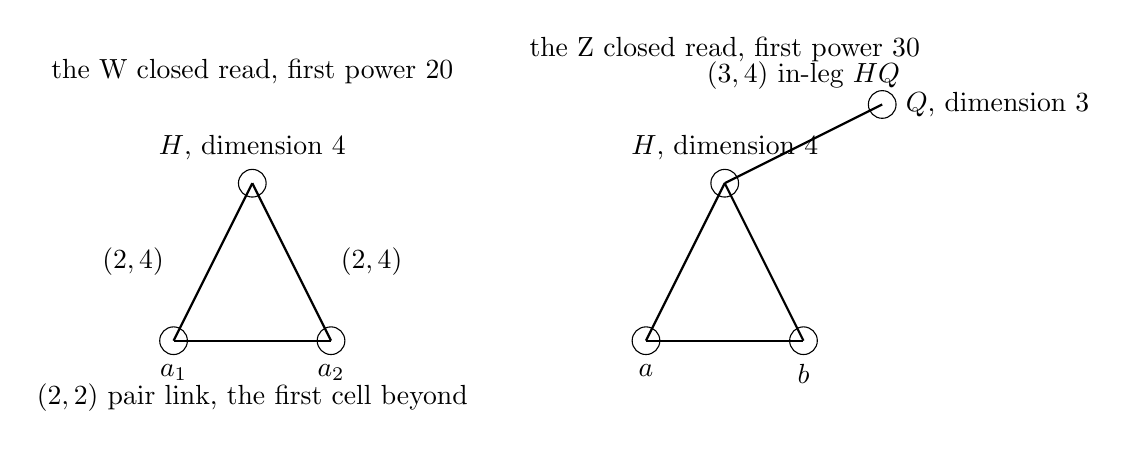
\begin{tikzpicture}[scale=1]
\filldraw[fill=white] (1,2) circle (5pt) node[above=5pt] {$H$, dimension 4};
\filldraw[fill=white] (0,0) circle (5pt) node[below=5pt] {$a_1$};
\filldraw[fill=white] (2,0) circle (5pt) node[below=5pt] {$a_2$};
\draw[thick] (1,2) -- (0,0); \draw[thick] (1,2) -- (2,0); \draw[thick] (0,0) -- (2,0);
\node at (1,0) [below=12pt] {$(2,2)$ pair link, the first cell beyond};
\node at (0,1) [left] {$(2,4)$}; \node at (2,1) [right] {$(2,4)$};
\node at (1,3) [above=4pt] {the W closed read, first power $20$};
\filldraw[fill=white] (7,2) circle (5pt) node[above=5pt] {$H$, dimension 4};
\filldraw[fill=white] (6,0) circle (5pt) node[below=5pt] {$a$};
\filldraw[fill=white] (8,0) circle (5pt) node[below=5pt] {$b$};
\filldraw[fill=white] (9,3) circle (5pt) node[right=5pt] {$Q$, dimension 3};
\draw[thick] (7,2) -- (6,0); \draw[thick] (7,2) -- (8,0); \draw[thick] (6,0) -- (8,0); \draw[thick] (7,2) -- (9,3);
\node at (8,3) [above=2pt] {$(3,4)$ in-leg $HQ$};
\node at (7,3) [above=12pt] {the Z closed read, first power $30$};
\end{tikzpicture}\caption{The two closed-genre reads: the W read over a (2,2) pair link and two (2,4) legs, and the Z read with its (3,4) in-leg, the two cells beyond the dock and the leg.}\end{figure}
\end{chproof}
\par\medskip\noindent{\itshape The carriers named, the next chapter is the chapter of their genre.}\label{narr:close:6-2}\par
\section{The instrument tables of this Part}\label{mod:VIII-L-the-instrument-tables-at-the-repository}
\chdesig{8-L}{}{VIII-L-the-instrument-tables-at-the-repository}{VIII-L-the-instrument-tables-at-the-repository}
\begin{chtable}[The instrument tables of this Part]\label{box:VIII-L-the-instrument-tables-at-the-repository:1}
This Part lists 13 instrument chapters, printed among the instruments at the end of this compendium as chapters~\ref{mod:VI-2a-2-4-genre-the-carrier-legs-and-the-neutral-lepton-ports} to~\ref{mod:VI-9-D543021-vcst-t1}, and the table beneath names each one with its key cells.
\end{chtable}
\chstanding{instrument}
\chdeps{Definitions 1.1 to 1.6}{no theorem beyond it at this release}
The listing moves no cell and states no result of its own. Each instrument stands at the repository as its chapter stood at the previous release of this compendium, and its tables are read there.
\begin{chbridge}
The tables listed here are instruments of this compendium, each listed under the title of its chapter.
\end{chbridge}
\begin{chproof}[instrument]
The listing in full. For each instrument chapter, printed among the instruments at the end of this compendium, the table gives its title, the result boxes it carries, the standing of each box with its citation, and the count of objects its certificate sentence names where it prints one.
{\small
\begin{longtable}{p{38mm}p{63mm}p{30mm}p{14mm}}
\hline
chapter & results & standing & objects \\
\hline
\endhead
The (2,4) genre: the carrier legs and the neutral-lepton ports & The (2,4) genre chapter & instrument & -- \\
The (2,4) genre: the carrier legs and the neutral-lepton ports & the text of the chapter & see its text & -- \\
The (2,4) genre: the carrier legs and the neutral-lepton ports & the text of the chapter & see its text & -- \\
The (2,4) genre: the carrier legs and the neutral-lepton ports & the text of the chapter & see its text & -- \\
The (2,4) genre: the carrier legs and the neutral-lepton ports & The open port and its conjugate end & theorem & 12 \\
The (2,4) genre: the carrier legs and the neutral-lepton ports & The weak angle as the ratio of the (2,3) and (2,4) dressings & open result & 519 \\
The charged and neutral currents & The currents chapter & instrument & -- \\
The charged and neutral currents & The neutral current as the Z read at the whole sinks & theorem & 36 \\
The charged and neutral currents & The charged current as the hub step at every sink & open result & 182 \\
The Fermi constant and the muon decay & The Fermi-constant chapter & instrument & -- \\
The Fermi constant and the muon decay & The Fermi constant as the W word office at low transfer & open result & 12 \\
The electroweak table & The electroweak table & instrument & -- \\
The electroweak table & The electroweak breaking as the stabilizer of the vacuum register & conditional theorem & 6 \\
\hline
\end{longtable}
}
The rule that produced it. Every chapter of this Part whose first standing beyond a placeholder reads instrument is printed among the instruments at the end of this compendium with its tables, and its key cells are the titles of its boxes, its standing lines and its certificate count, read from its text as it stood at the previous release.
No derivation stands in this chapter; the tables stand at the repository.
\emph{Check.} Every file listed was re-hashed at the repository and read the same as its recorded hash, and the listing was re-cut from the files by a second route.
Nothing stands open at this listing. At this release four results of this Part are re-graded at their chapters: the hub step as the weak interaction (the chapter 8-1), its open result closed as a conditional theorem at the decay path; the W and the Z (the chapter 8-2), the Z read re-posed at the route identity; the neutral lepton (the chapter 8-2b), the released body closed as a conditional theorem at the nested cross; beta decay (the chapter 8-8), closed as a theorem at the literal closure reading.
\end{chproof}
\label{chend:VIII-L-the-instrument-tables-at-the-repository}
\section{The neutral lepton: the hub unit with its legs open}\label{mod:VI-2b-neutral-lepton-the-hub-unit-with-its-legs-open}
\chdesig{8-2b}{6-2b}{VI-2b-neutral-lepton-the-hub-unit-with-its-legs-open}{VI-2b-neutral-lepton-the-hub-unit-with-its-legs-open}
\label{narr:open:6-2b}Theorem~162.1 reads the released body as one anatomy, the hub unit with its legs open, an open result, and Theorem~162.2 gives the census of the neutral sinks.
\begin{chconditional}[The released body as one anatomy]\label{box:VI-2b-neutral-lepton-the-hub-unit-with-its-legs-open:1}
Conditional on the results this theorem rests on at their own standing, as its derivation names them.
The released object of every generation is the cross nested at the depth one less, read at the order two through the hub: the body released at the second generation, four sites at the measure twenty-eight, is isomorphic at the labeled links to the hub assembly the nesting adds at the first depth by the least map of its sites, the body released at the third generation to the assembly added at the second depth by the corresponding map, every one of the three (2,4) hub links at the readability order two and the (2,2) pair at the order one at both objects at both generations, every link at the dressing of its genre at both spellings, and the body released at the first generation empty against the empty cross nested at the depth zero, the bare core nesting no cross; at the reading that gives the empty depth a body the first generation parts, both faces printed. The body released in every charged-lepton decay is thereby one anatomy, the junction assembly with its core in-leg struck, four sites at the measure twenty-eight, as the previous open result named it, and its identity with the nested cross of the next depth is the theorem; neutrality remains typed at the sinks of the saturation as two open qubit ports under the adopted definition, the two sets of the previous reading parting at the typed webs docked at charge zero, and whether the released body is of the Dirac or of the Majorana kind is a reading of the act and not an output of the construction; the deciding table is re-derived in Lean.
\end{chconditional}
\chstanding{conditional theorem, built at the nested cross}
\chdeps{Definitions 1.1 to 1.6, Theorem 152.1, Theorems 196.1 and 196.2 and Open results 245.1 and 245.2, Theorem 245.3, Open results 245.4 to 245.8 and Theorem 245.9}{Theorem 166.1 and Open results 166.2 and 166.3 and Theorem 254.1}
The box names the thing a decay releases, not a new kind of object but a piece of the decaying web, the hub with its leaf pair and its odd leg, left with two valences free where its core and its leaf stood. Neutral means two open qubit ports, and the box says that this typing is not the same as reading zero charge at every web.
\begin{chconditional}[The neutral sinks census]\label{box:VI-2b-neutral-lepton-the-hub-unit-with-its-legs-open:2}
Under the site-97 closure cut at wave four and the adopted definition of open at the ports, the lowest neutral sink of the census, at wave two, is a web of three sites and two qutrit-qubit links, among one hundred eighty-five neutral sinks counted wave by wave; the two neutral objects of the prior release stand among the sinks as one.
\end{chconditional}
\chstanding{conditional theorem, named at two ports}
\chdeps{Definitions 1.1 to 1.6, Theorem 152.1, Theorems 196.1 and 196.2 and Open results 245.1 and 245.2, Theorem 245.3, Open results 245.4 to 245.8 and Theorem 245.9}{Theorem 166.1 and Open results 166.2 and 166.3 and Theorem 254.1}
The second box is a count, among every sink the saturation reaches by wave four, those with exactly two open qubit ports are counted and the smallest is named as a web, with no name of the literature attached to it.
\begin{chbridge}
What this chapter calls the released body the literature calls the light neutral lepton released beside the charged one at its decay, and the hub unit with its legs open its neutral partner in the weak doublet. The correspondence is by name, and no mass, count or measured value enters this page.
\end{chbridge}
\begin{chproof}[exact]
The premises of the first box are the saturation with its waves and sinks of chapter 1-5, a theorem, the lepton ladder as hub assemblies of chapter 5-10, a theorem, and the unstable rows of chapter 8-3, an open result. The chain from the axiom to this chapter is eight chapters long. The exact part first. From the muon web, by the inverse hub step at its hub (the edge from the muon vertex to the electron vertex of the move graph of the first chapter of this Part), we obtain the released object, listed as a table here, the drawing means of this compendium admitting no picture.
\begin{center}\small
\begin{adjustbox}{max width=\linewidth}\begin{tabular}{llll}
\hline
site & dimension & link & genre \\
\hline
$H_2$ & 4 (the hub) & $H_2 b_1$ & (2,4) \\
$b_1$ & 2 (a leaf) & $H_2 b_2$ & (2,4) \\
$b_2$ & 2 (a leaf) & $H_2 b_3$ & (2,4) \\
$b_3$ & 2 (the odd leg) & $b_1 b_2$ & (2,2) \\
\hline
\end{tabular}\end{adjustbox}

The released body. The hub with its leaf pair and its odd leg, the in-link valence freed at the hub where the core stood and the pairing valence freed at the odd leg where the leaf stood.
\end{center}
From the four links, by the rank, we obtain the measure of the box,
\begin{equation}
28 = 2 \cdot 4 + 2 \cdot 4 + 2 \cdot 4 + 2 \cdot 2 ,
\end{equation}
and the same web is released at every one of the inverse edges of the move graph that release one. From the two free valences at the qubit ends, by the adopted definition of open, we obtain the typing of the box, two open qubit ports, neutral.

From the webs whose charge the construction establishes, by reading the established charge and the dock-free read side by side, we obtain the parting of the box, the established charge, typed at one hundred forty webs, reads zero at every one of them while the set of webs reading zero at the dock-free read holds more, so neutrality typed at the two ports and the dock-free read part at the typed webs docked at charge zero. At the readings beside, the cross-core pair released by the inverse hub step at the muon edge is two bodies at all nine pairs of readings and one body at none. The light neutral body as the Higgs link with its ports open parts from the charged partner at the structural reading. The Majorana-or-Dirac reading at the ports is a reading of the act and not an output of the literal clause. The baseline webs at the neutral sinks are unbuilt at the truncation, and one further reading takes the released object as one anatomy and not as the nesting of its generation.

The census part. From the sinks of the site-97 closure cut at wave four, by typing every sink at its open qubit ports, we obtain the four kinds, one sink beyond two ports, 5455 charged, 38700 dark with no open dock end, and the neutral sinks at two open dock ends,
\begin{equation}
185 = 1 + 6 + 178
\end{equation}
by wave two, three and four. By hub count they sort as 4, 4, 32, 56, 57, 20 and 12 at zero to six hubs. The smallest case. At wave two the one neutral sink is the web numbered 19, three sites $s_0$, $s_1$ of dimension 2 and $s_2$ of dimension 3 with the two links $s_0 s_2$ and $s_1 s_2$ of genre (2,3), its two open ports the docks at $s_0$ and $s_1$, reached from a root that is a pair ket by one attachment and one reversal. The nearest neutral sinks at one port fewer and at one port more are none. From the two neutral objects of the earlier result, by isomorphism against the sinks, we obtain one of them among the sinks (the triangle of dimensions 4, 2, 2 with two pendant ports, at one sink) and the other at none.

\emph{Check.} The eleven intermediate tables of the first box are cited at a note, the released object and its measure are taken from the result on the two neutral objects, which prints the same web at the muon edge, and the typing from the census result. Where a step of the first box is not carried by those two results it is stated and not derived here. What would have broken the census, the open definition replaced by the open dock ends or by the free valence at the qubit sites moves the port counts and leaves the lowest sink the same web. The twin closure at the web cap gives 62 neutral sinks with a different lowest sink at wave three. Each result was reproduced by an independent route, two engines at every capture byte for byte, its counter-tests at their pinned letters and its controls the same at both routes.
The mixing at the open ports is the matter of the mixing chapter of this Part.
\chcert{185}
\end{chproof}
\label{chend:VI-2b-neutral-lepton-the-hub-unit-with-its-legs-open}
\par\medskip\noindent{\itshape With the neutral lepton read, the next chapter pairs it with the charged one in the doublet.}\label{narr:close:6-2b}\par
\section{The doublets, handedness and parity violation}\label{mod:VI-3-doublets-handedness-and-parity-violation}
\chdesig{8-3}{6-3}{VI-3-doublets-handedness-and-parity-violation}{VI-3-doublets-handedness-and-parity-violation}
\label{narr:open:6-3}Theorem~163.1 gives the weak doublet at the internal ends of the leptons, Open result~163.2 the isospin sign as the dart charge minus half the weight, Theorem~163.3 the doublet count at the cross core, and Open result~163.4 the doublet as the set of sinks at every label and the sum at the set.
\begin{chconditional}[The weak doublet at the internal ends of the leptons]\label{box:VI-3-doublets-handedness-and-parity-violation:1}
Under the sixteen rows of chapter 4-1, the weights of chapter 4-2 and the open-end census of chapter 4-3, the weak doublet of a lepton is the one internal read at the odd leg of its junction: the one-act read that opens the odd-leg qubit copy is a doublet of the internal su(2) at the centre weight $n - 3$ and $6T_3 - 3$ with the two-ality $d = 1$, at the electron, the muon and the tau alike, every other internal read being closed under the join, closed at its dimension-four far end or washed at the (2,2) pair. The two charged-lepton rows of the sixteen are re-reached, the L row by the internal doublet read with the one-dock read beside it and the R row by the two-dock read, a singlet at $d = 0$; the two reads commute, the chirality from the dock link and the internal doublet from the hub leg varying independently.
\end{chconditional}
\chstanding{conditional theorem}
\chdeps{Definitions 1.1 to 1.6, Theorems 9.1 to 9.7 and Open result 9.8, Theorems 18.1 to 18.4 and Open results 18.5 and 18.6, Theorems 64.1 and 64.2, Theorems 65.1 and 65.2, Open results 66.1 to 66.3, Theorem 66.4 and Open result 66.5 and Open results 241.1 and 241.2, Theorems 241.3 and 241.4 and Open results 241.5 to 241.7}{Open results 72.1 to 72.3, Theorem 72.4 and Open result 72.5, Theorem 73.1 and Open results 73.2 and 73.3, Theorems 74.1 to 74.4 and Open result 74.5, Open result 163.4 and Theorems 200.1 to 200.3 and Open result 200.4}
Of all the one-act reads a lepton admits at its internal links, exactly one, at the odd leg of its junction, is a doublet, at all three charged leptons alike. The handedness comes from the dock, so chirality and isospin are carried by two reads that commute.
\begin{chwall}[The isospin sign as the dart charge minus half the weight]\label{box:VI-3-doublets-handedness-and-parity-violation:2}
The isospin component a lepton occupies, read as the dart charge, the charge of a directed edge, minus half the weight at the internal end, is an exact object at every body. On the one face the electron and the neutral body agree with the sixteen rows at the component, the sign and the weight; on the other face the muon and the tau part from them, the parting at the muon.
\end{chwall}
\chstanding{open result, built and not closed}
\chdeps{Definitions 1.1 to 1.6, Theorems 9.1 to 9.7 and Open result 9.8, Theorems 18.1 to 18.4 and Open results 18.5 and 18.6, Theorems 64.1 and 64.2, Theorems 65.1 and 65.2, Open results 66.1 to 66.3, Theorem 66.4 and Open result 66.5 and Open results 241.1 and 241.2, Theorems 241.3 and 241.4 and Open results 241.5 to 241.7}{Open results 72.1 to 72.3, Theorem 72.4 and Open result 72.5, Theorem 73.1 and Open results 73.2 and 73.3, Theorems 74.1 to 74.4 and Open result 74.5, Open result 163.4 and Theorems 200.1 to 200.3 and Open result 200.4}
The sign inside the doublet is an integer in sixths from two counts of the web, agreeing with the sixteen rows at the first generation and parting at the second and third.
\begin{chconditional}[The doublet count at the cross core]\label{box:VI-3-doublets-handedness-and-parity-violation:3}
Under the statistics from the odd-cycle sign, the doublet swap at the generic qubit read and the roster of bodies, the doublet count rule holds at the cross core of the three cross-core webs, where the depths read odd and the swap is met at the eighteen objects.
\end{chconditional}
\chstanding{conditional theorem}
\chdeps{Definitions 1.1 to 1.6, Theorems 9.1 to 9.7 and Open result 9.8, Theorems 18.1 to 18.4 and Open results 18.5 and 18.6, Theorems 64.1 and 64.2, Theorems 65.1 and 65.2, Open results 66.1 to 66.3, Theorem 66.4 and Open result 66.5 and Open results 241.1 and 241.2, Theorems 241.3 and 241.4 and Open results 241.5 to 241.7}{Open results 72.1 to 72.3, Theorem 72.4 and Open result 72.5, Theorem 73.1 and Open results 73.2 and 73.3, Theorems 74.1 to 74.4 and Open result 74.5, Open result 163.4 and Theorems 200.1 to 200.3 and Open result 200.4}
The third box counts doublets at the shared core of the three cross-core webs, the rule met at all eighteen objects.
\begin{chbridge}
What this chapter calls the internal doublet read the literature calls the weak isospin doublet of the left-handed leptons, the dock read its chirality and the component in sixths its third isospin component, the nearest objects. The correspondence is by name.
\end{chbridge}
\begin{chproof}[census]
The premises are the link and its six genres of chapter 1-2, the reads and the Born count of chapter 1-3 and the moves of chapter 1-4, definitions, and the sixteen rows, the weights and the open-end census of chapters 4-1 to 4-3, theorems and open results. The chain from the axiom to this chapter is seven chapters long. The set counted is the set of one-act reads at the internal links of the three lepton bodies, generated by opening each internal link at its qubit copy with the hub leg entered at its ket copy and the join kept. The property tested is whether the read is a doublet of the internal su(2). By kind the reads sort into the one doublet read per body, at the odd-leg copy of the junction, with the two-ality 1 and the weights $n - 3$ and $6T_3 - 3$, and the rest, closed under the join, closed at a dimension-four far end, or washed at the (2,2) pair. The smallest case. At the electron the one-dock read beside the doublet read carries the weight $n - 3$ equal to the row $6Y$, the dock count 1 the chirality L. The two-dock read is the singlet at $d = 0$, $6T_3 = 0$ and $n - 6$ by the exchange sign at the two dock ends, the row R. The two reads act on distinct links with disjoint open sets, so they commute, and the sixteen rows are re-reached at their ordinals, 16 of 16.

From the dart charge at the dock face and the half-weight at the internal end, by subtraction, the components at the four bodies are
\begin{equation}
-6 - (-3) = -3, \qquad 0 - (-3) = 3, \qquad -12 - (-3) = -9, \qquad -18 - 0 = -18 ,
\end{equation}
at the electron, the neutral body, the muon and the tau, every sign the odd-leg state, the electron and the neutral body agreeing with the sixteen rows and the muon and the tau parting. The doublet count rule is met at the cross core of the three cross-core webs at 18 of 18 objects, the depths reading odd there.

\emph{Check.} At the reading with the hub never entered no internal read is a doublet at any body, printed beside. The neutral body under the kept join carries no internal doublet at either reading. The counts of the closed and washed reads stand at the tables of the entry and are not re-listed here. Each result was reproduced by an independent route, two engines at every capture byte for byte, its counter-tests at their pinned letters and its controls the same at both routes.
The doublet content under the weights does not follow the dock count, and the component at the muon and the tau parts from the sixteen rows.
\chcert{16}
\end{chproof}
\label{chend:VI-3-doublets-handedness-and-parity-violation}
\subsection{The doublet as the set of sinks at every label}\label{mod:VI-3-D538842-w-dbcl}
\begin{chwall}[The doublet as the set of sinks at every label and the sum at the set]\label{box:VI-3-D538842-w-dbcl:1}
At every label of the representation census the set of stable webs, the sinks, at that label is a doublet set and the catalogued body lies inside it, but the sum over the set is nonzero at every label. On the one face a doublet member is found at every one of the three labels with the body inside its set; on the other face the four sums over the words the set reaches read 3, 189, minus 3 and 0 at every label where zero was asked, the first label without being the label one.
\end{chwall}
\chstanding{open result, built and not closed}
\chdeps{Definitions 1.1 to 1.6, Open results 66.1 to 66.3, Theorem 66.4 and Open result 66.5 and Theorem 163.1, Open result 163.2 and Theorem 163.3}{no theorem beyond it at this release}
The box re-reads the doublets of this chapter at the level of whole stable webs, the sinks of the saturation sorted by the number of their hubs, which the compendium reads as the generation, form three sets, each set contains doublet members and the cataloged lepton of that generation, and the anomaly-like sums that an earlier reading asked to vanish do not vanish over any of the three sets.
\begin{chbridge}
What this chapter calls the sink set at a label the literature calls the multiplet of a generation, and the doublet member its left-handed doublet, the nearest objects. The correspondence is by name.
\end{chbridge}
\begin{chproof}[finite computation]
The premises are the doublets of this chapter, a theorem, the representations from the open-end census of chapter 4-3, a theorem, and the saturation with its sinks of chapter 1-5, a theorem. The chain from the axiom to this result is eight chapters long. The procedure. The input is the union of 22302 saturated sinks and its 744 lepton-form sinks. The enumeration sorts them by hub count, the label of the generation,
\begin{equation}
744 = 48 + 156 + 231 + 300 + 9
\end{equation}
at zero, one, two, three and more hubs. The test at each sink is its typing at the dock rule, a doublet of color one, a weak singlet of color one, or a vanishing content. The aggregation is the four sums over the words the set reaches. The smallest instance is the set at the label one,
\begin{equation}
156 = 35 + 54 + 67 ,
\end{equation}
thirty-five doublet members (the first in the order of the material a proton sink at one dock), fifty-four weak singlets and sixty-seven at a vanishing content. The cataloged electron, located among them by isomorphism at two docks, lies inside the set as a weak singlet and inside the doublet subset not. At the labels two and three the doublet members are 60 of 231 and 129 of 300, the first a proton sink and a tau-row sink, and the cataloged bodies of those generations lie inside the doublet subset.

From the members at a label, by the words the set reaches at the adopted typing, two words at each label (89 of 156, 138 of 231 and 300 of 300 members at a word), and by the four sums with the weights 3 per open qubit end and minus 2 per open qutrit end, we obtain at every label the same four values, the linear sum, the cubic sum and the two mixed sums,
\begin{equation}
\ell = 3, \qquad c = 189, \qquad m_{2} = -3, \qquad m_{3} = 0 ,
\end{equation}
zero at 0 of 3 labels. Over the doublet members alone the sums read minus 3, minus 27, minus 3 and 0, and over the members with multiplicity 219, 10719, minus 105 and 0 at the label one, nonzero likewise. So the doublets clause holds, the sums clause fails, and the open result is named at the label one.

\emph{Check.} Reading the label by the attach-site count in place of the hub count sorts the sinks as 98, 488, 154, 2 and 2 and leaves the board labels present and the sums nonzero. The cataloged body is inside the doublet subset proper at two of the three labels. The result was reproduced by an independent route, two engines at every capture byte for byte, its counter-tests at their pinned letters and its controls the same at both routes.
The sum over the doublet set stays nonzero at every label.
\chcert{744}
\end{chproof}
\label{chend:VI-3-D538842-w-dbcl}
\par\medskip\noindent{\itshape The doublets read, the next chapter reads the two currents that run between their members.}\label{narr:close:6-3}\par
\section{The weak angle}\label{mod:VI-6-weak-angle}
\chdesig{8-6}{6-6}{VI-6-weak-angle}{VI-6-D539645-w-wbsq}
\label{narr:open:6-6}Theorem~164.1 reads the weak angle as the dock share, Open result~164.2 as the office of the W word, Open result~164.3 from the stabilizer weights, Open result~164.4 per family at the tau sink, and Theorem~164.5 as the ratio of offices at the Z body.
\begin{chconditional}[The weak angle as the dock share]\label{box:VI-6-weak-angle:1}
Under the results it rests on, the dock share is one structure at the W body, the Z body and their joined web: the two bodies, the roster W word and the roster Z word, are each a seeded sink at wave zero at both stop readings, five sites and four links at the genres qutrit-qubit twice and ququart-qubit twice, the measure twenty-eight, isomorphic by an explicit map, each with a total end set of eight ends and the dock ends of its two qutrit-qubit links; the dock share is a per-link quotient, additive over the links and unmoved by a shared site.
\end{chconditional}
\chstanding{conditional theorem}
\chdeps{Definitions 1.1 to 1.6, Theorems 185.1 to 185.12 and Theorems 197.1 to 197.4 and Open result 197.5}{Theorem 164.5, Chapter 8-6 and Theorem 255.1}
The box says that the quantity the compendium reads as the weak angle, the share of a body's ends that are dock ends, is the same structure whether read at the W, at the Z or at the two joined, because it is computed link by link and the two bodies are the same web.
\begin{chwall}[The weak angle as the office of the W word]\label{box:VI-6-weak-angle:2}
The count readings of the coupling read rule, met again from the pair ket at the qutrit-qubit read links of the W word and the Z word, are seventeen over thirty-six at the whole and fourteen over thirty-six at the cut, equal to the established cells at both words. On the one face the count faces are re-met from the pair ket and the office of the W word is the Born square of its first power; on the other face the step from the office of the W word to the square of the angle is refused at its first step, the third of five, the closed read, since the first power 28 over either unit is named the closed read by no established clause.
\end{chwall}
\chstanding{open result, built and not closed}
\chdeps{Definitions 1.1 to 1.6, Theorems 185.1 to 185.12 and Theorems 197.1 to 197.4 and Open result 197.5}{Theorem 164.5, Chapter 8-6 and Theorem 255.1}
The second box tries to derive the squared angle from the office rule applied to the W word, and finds the rule licenses only its first two steps there. The count face of the pair ket and the first power of the word are two different numbers and no clause makes one the other.
\begin{chwall}[The weak angle from the stabilizer weights]\label{box:VI-6-weak-angle:3}
The end-face figure of the angle from the stabiliser weights is three over eight at the dock reading and two over five at the hub reading, an exact rational; on the other face the established running rows carry that figure at no rung.
\end{chwall}
\chstanding{open result, built and not closed}
\chdeps{Definitions 1.1 to 1.6, Theorems 185.1 to 185.12 and Theorems 197.1 to 197.4 and Open result 197.5}{Theorem 164.5, Chapter 8-6 and Theorem 255.1}
The third box gives a figure for the angle from the norm ratio of two directions of the register, and finds it at no rung of the running.
\begin{chwall}[The weak angle per family at the tau sink]\label{box:VI-6-weak-angle:4}
The weak angle per family at the tau sink stands as an open result named at its second face: the three family shares read two thirds, one third and one half at the electron, the muon and the tau with the family average one half.
\end{chwall}
\chstanding{open result, built and not closed}
\chdeps{Definitions 1.1 to 1.6, Theorems 185.1 to 185.12 and Theorems 197.1 to 197.4 and Open result 197.5}{Theorem 164.5, Chapter 8-6 and Theorem 255.1}
The fourth box reads the share family by family. The tau share and the average equal the cell of the next section, the electron and the muon do not.
\begin{chbridge}
What this chapter calls the dock share, the count face and the office ratio the literature calls the squared sine of the weak mixing angle, each the nearest object. The correspondence is by name, and the value of the angle is displayed nowhere in this chapter.
\end{chbridge}
\begin{chproof}[finite computation]
The premises are the mass unit and the first power of chapter 8-1, a theorem, the three generations as attach sites of chapter 8-4, a theorem, and the W word of chapter 6-2, an open result. The chain from the axiom to this chapter is eight chapters long. The procedure of the second box, the input is the W word, five sites of dimensions 4, 2, 3, 2, 4 and four links, and the Z word, the same web. The enumeration lists the reads the read rule admits at end product at most 6, the two qutrit-qubit links at the middle site. The test poses the pair ket on the common support of dimension 2 and counts the 36 pair letters of the qutrit end and the qubit end by the amplitude of each. The aggregation is the count face. From the 36 pair letters, 17 nonzero at the whole and 14 at the cut, we obtain
\begin{equation}
\frac{17}{36}, \qquad \frac{14}{36} = \frac{7}{18}, \qquad \Bigl(\frac{17}{36}\Bigr)^{2} = \frac{289}{1296}, \qquad \Bigl(\frac{7}{18}\Bigr)^{2} = \frac{49}{324} ,
\end{equation}
with the sector sums one sixth, one twelfth, zero and three quarters at the weight sum 1, equal to the established cells of the two-read entry and the coupling-read entry at both words. From the first power of the W word, the rank 28 at the dressing 1, by the Born square over the unit 201 at the hub face and 67 at the dock face, we obtain the office
\begin{equation}
\Bigl(\frac{28}{201}\Bigr)^{2} = \frac{784}{40401}, \qquad \Bigl(\frac{28}{67}\Bigr)^{2} = \frac{784}{4489} ,
\end{equation}
equal to the office, support and Born tables of the office entry at both words. The five steps of the office rule, the body, the support, the closed read, the Born square and the unit, are licensed at 5 of 5 when the closed read is the first power and at 2 of 5 when it is the count face, the third step refuses, the parting of the box, with both objects printed,
\begin{equation}
\frac{289}{1296} \neq \frac{784}{40401}, \qquad \frac{49}{324} \neq \frac{784}{4489} .
\end{equation}

For the first box, from the two words as seeded sinks at wave zero at both stop readings, by listing their ends, we obtain eight ends at each and the dock ends of the two qutrit-qubit links. The dock share is the per-link quotient, additive over the links and unmoved by the shared site, one structure at the W, at the Z and at the joined web. The Z word is tied to the W word at 17 of 17 register cells, the difference zero and the ratio one at every one, the measure, the rank and the first power 28. At the qutrit-qubit genre the whole 36, the cut 24, the common-support register 16 and the two links. At the ququart-qubit genre the whole 64, the cut 45, the register 16 and the two links. The count faces and the offices. The register of the Z body is the Born count of the qutrit-qubit genre from its coherent sector counts at the basis gains,
\begin{equation}
319 = 79 \cdot 1 + 48 \cdot 2 + 42 \cdot 3 + 3 \cdot 6 .
\end{equation}
For the third box the end-face figure is the norm ratio of the third-component direction against the charge under the plain trace form on the register of the split at the matched scale, three over eight at the dock reading and two over five at the hub reading, unmoved under the composed map at every rung and carried by the running rows at none. For the fourth box the shares read two thirds, one third and one half with the average one half.

\emph{Check.} What would have broken the second result, the ququart-qubit legs give the count faces 22 over 64 and 19 over 64 and the closed-read genre of the carrier entry 4 over 16 and 3 over 16, neither the office. The Z word tried in place of the W word gives every cell the same. Each result was reproduced by an independent route, two engines at every capture byte for byte, its counter-tests at their pinned letters (four at the office rule) and its controls the same at both routes (ten there).
The step from the office of the W word to the square of the angle stays refused at its third step, and the figure from the stabilizer weights stands at no rung of the running, which is the matter of chapter 5-7.
\chcert{36}
\end{chproof}
\label{chend:VI-6-weak-angle}
\subsection{The weak angle as the ratio of offices at the Z body}\label{mod:VI-6-D539022-wazb-t1}
\begin{chconditional}[The weak angle as the ratio of offices at the Z body]\label{box:VI-6-D539022-wazb-t1:1}
Under the results it rests on, the office of the W word and the office of its two-line read are both defined at the register of the Z body, and their ratio is the exact rational one half, one cell at the Z body: equal at the Z-body register, at the hub unit and at the dock unit, the unit cancelling; equal at the three count-level forms of the weights; and equal at both orthogonal-sum readings.
\end{chconditional}
\chstanding{conditional theorem}
\chdeps{Definitions 1.1 to 1.6, Open results 159.1 and 159.2 and Theorem 164.1 and Open results 164.2 to 164.4}{no theorem beyond it at this release}
The box divides the Born square of the one-line read by the Born square of the two-line read at one register, the register the Z body reaches, and finds one half, the same number whichever unit, count-level weighting or orthogonal reading is chosen. The tau share and the family average of the chapter above equal it, the electron and muon shares do not.
\begin{chbridge}
What this chapter calls the ratio of the two offices the literature calls the squared cosine of the weak mixing angle, its complement the squared sine, and the Z body the Z boson, the first two the nearest objects and the last by name. The correspondence is by name, and no value of the angle is displayed here.
\end{chbridge}
\begin{chproof}[census]
The premises are the W and the Z of chapter 6-2, an open result, and the weak angle chapter above. The chain from the axiom to this result is nine chapters long. The exact part first. From the first power of the W word 28, re-met at five sources, and the register the Z body reaches, the Born count 319 of the qutrit-qubit genre, by the Born square, we obtain the office of the W word. From the orthogonal two-line sum $28\sqrt{2}$ at the count form, by the same square, the office of the Z read, and by division their ratio,
\begin{equation}
\frac{784}{101761}, \qquad \frac{1568}{101761}, \qquad \frac{784}{1568} = \frac{1}{2} ,
\end{equation}
with the complement one half, the inverse 2 and the square polarity three quarters beside. At the hub unit the two offices read 784 and 1568 over 40401 and at the dock unit over 4489, the ratio one half at every register.

The census part. The set counted is the grid of forms, readings and registers at which the two offices are defined, 99 cells of the office table. The property tested is whether the ratio equals the cell of the box, one half. By kind. At the three registers 3 of 3 equal. At the three count-level forms, the count, pair and sup-pair forms, 3 of 3. At the two orthogonal-sum readings 2 of 2. At the three forms beyond the count level the ratio parts, one seventeenth, one thirty-seventh and one tenth at the amplitude weights and one fifth, one seventh and one quarter at the Born weights, the first parting the sup-near form at one seventeenth. At the two amplitude-sum readings it parts, one quarter at the count-level forms. The smallest case is the count form at the orthogonal reading at the Z-body register, the display above. From the three family shares, by comparison, we obtain the tau share one half and the family average one half equal to the cell, the electron share two thirds and the muon share one third parting.

\emph{Check.} The Z body is the W word at 17 of 17 register cells and isomorphic to it at the identity map, so the two offices are defined at one register. The partings beyond the count level and at the amplitude readings are printed beside. The result was reproduced by an independent route, two engines at every capture byte for byte, its four counter-tests at their pinned letters and its twelve controls the same at both routes.
The comparison of the cell with the measured angle stands at the comparison table alone.
\chcert{99}
\end{chproof}
\label{chend:VI-6-D539022-wazb-t1}
\section{The weak angle as the office of the W word pair ket}\label{mod:VI-6-D539645-w-wbsq}
In the electroweak theory the weak mixing angle fixes the ratio of the W and the Z masses at the tree level and the relative strength of the neutral and the charged currents; its sine squared is the ratio of the squared couplings, a free parameter of the Standard Model fixed by measurement and not by the theory \cite{Glashow1961,Weinberg1967,Salam1968}. The weak angle is introduced at section~\ref{mod:VI-6-weak-angle}, the W and the Z at section~\ref{mod:VI-2-w-and-the-z-and-their-masses} and the body-alone office rule at section~\ref{mod:VIII-2-body-alone-office-rule}.
The count face of the pair ket at the (2,3) read link of the W word, 17 over 36 at the whole and 14 over 36 at the cut, agrees with the established values at 4 of 4 links of the word, the Z word tied at 4 of 4; but it is no first power of the body-alone rule read at the word, so the weak angle is not the office of the W-word pair ket at any of the three clauses posed.
The rule names the first power 28 at the word, from the measures 8, 6, 6 and 8 at the dressing one with nothing struck and the pair part 784 by the two-read identity; the dark set is the two (2,4) legs and the closure 10241 over 3645000 plus 98 over 50625 root 2 at the swapped weight of the (2,4) genre, the office 2857690241 over 3645000 plus 98 over 50625 root 2 agreeing with the W read and the W word result. At the register 36 of the read link the first power reads 7 over 9 against the count faces 17 over 36 and 7 over 18, and the office over the register squared is an element of the field with a root 2 part against the rational Born squares 289 over 1296 and 49 over 324; at the read link alone the first power is 6 and the office 36, parting likewise with the dark set empty there, at the two read links 12 and 144, and at the segment reading the word is carried at no read. The Born squares are exact values at both faces, and a grid of 72 readings meets at none.
The result is an open one, an open result: the stronger statement is not met at the whole face nor at the cut face, and the weaker statement is named; no comparison with observation is made here.
What stays open is whether the Born square at the word is an output of the body-alone rule, which no result settles at this stage; the weak angle at the one value of the Z body (section~\ref{mod:VI-6-D539022-wazb-t1}) and the Z read of the W word (section~\ref{mod:VI-2-w-and-the-z-and-their-masses}) stand beside at their own sections.
\par\medskip\noindent{\itshape The angle read, the next chapter reads the mixing between the generations.}\label{narr:close:6-6}\par
\section{Mixing, the washed overlap and the CKM block}\label{mod:VI-7-mixing-the-washed-overlap-and-the-ckm-block}
\chdesig{8-7}{6-7}{VI-7-mixing-the-washed-overlap-and-the-ckm-block}{VI-7-D543182-w-mxog}
\label{narr:open:6-7}Theorem~166.1 reads mixing as the overlap of the corner frame with the depth eigenbasis, Open result~166.2 as the corner-frame overlap through the W, Open result~166.3 the mixing phase at the four-cycle and the dock weights, Open result~166.4 the mixing as the sink-basis overlap, Open result~166.5 as the washed overlap of the arm reads, and Open result~166.6 the quark mixing block at the read sites.
\begin{chconditional}[Mixing as the overlap of the corner frame with the depth eigenbasis]\label{box:VI-7-mixing-the-washed-overlap-and-the-ckm-block:1}
If the generation label is the depth momentum, and under the rung reading of the polar-unitary entry and the open results it rests on, the rung basis of the three families is the eigenbasis of the depth step and the mixing is the overlap of the corner frame, an eigenbasis at a corner of a lattice cell, with it: the depth-step operator is factored by the Chinese remainder map into a qubit share and a qutrit share, the three characters of the qutrit share are the eigenvectors of the unit rung shift, and the overlap of the corner basis with that eigenbasis is unitary by construction at every admitted cell at both corner-basis readings, a permutation at none, with every squared modulus one third, the order-three Fourier matrix at every admitted frame, its phase a third of a turn or two thirds at every quartet and a half turn at none.
\end{chconditional}
\chstanding{conditional theorem}
\chdeps{Definitions 1.1 to 1.6, Theorems 162.1 and 162.2 and Theorems 197.1 to 197.4 and Open result 197.5}{Theorem 27.1, Open result 166.4, Open result 166.5, Open result 166.6, Chapter 8-7, Open result 168.1, Open result 169.1 and Theorem 254.1}
The box identifies the mixing with a change of basis, one basis is the corner frame a lepton web carries at its dark triangle, the other the eigenbasis of the step that moves a body one rung up its ladder. The matrix between them is the discrete Fourier transform of order three, every entry of squared modulus one third.
\begin{chwall}[Mixing as the corner-frame overlap through the W]\label{box:VI-7-mixing-the-washed-overlap-and-the-ckm-block:2}
The overlap of the corner frame with the rung basis read through the W is not unitary at the primary reading. On the one face the lepton overlap through the W at the hub face is defined at all nine pairs and the quark overlap at the dock face at six of nine; on the other face the first pair at which the quark overlap is undefined is the up-type first-generation element against its down-type partner, returning nothing through its dock, and the first row not summing to one is the electron row, the rows and columns summing to one at none of the six.
\end{chwall}
\chstanding{open result, built and not closed}
\chdeps{Definitions 1.1 to 1.6, Theorems 162.1 and 162.2 and Theorems 197.1 to 197.4 and Open result 197.5}{Theorem 27.1, Open result 166.4, Open result 166.5, Open result 166.6, Chapter 8-7, Open result 168.1, Open result 169.1 and Theorem 254.1}
The second box reads the same overlap not as a change of basis but through the W, as a two-point read between a flavor web and a mass web joined at the hub. The resulting matrix of squared moduli is defined but is not unitary, and the open result stands at the first row whose entries do not sum to one.
\begin{chwall}[The mixing phase at the four-cycle and the dock weights]\label{box:VI-7-mixing-the-washed-overlap-and-the-ckm-block:3}
The phase read at the four-cycle and the dock weights meets the measured entry at no reading.
\end{chwall}
\chstanding{open result, built and not closed}
\chdeps{Definitions 1.1 to 1.6, Theorems 162.1 and 162.2 and Theorems 197.1 to 197.4 and Open result 197.5}{Theorem 27.1, Open result 166.4, Open result 166.5, Open result 166.6, Chapter 8-7, Open result 168.1, Open result 169.1 and Theorem 254.1}
The third box reads a phase off the four-cycle of the joined web and the dock weights and finds it at no reading equal to the entry the construction carries.
\begin{chbridge}
What this chapter calls the overlap of the corner frame with the depth eigenbasis the literature calls the lepton mixing matrix, and the overlap of the quark arm basis the quark mixing matrix of Cabibbo, Kobayashi and Maskawa, the nearest objects. The correspondence is by name, and no angle, phase or figure is displayed at this page.
\end{chbridge}
\begin{chproof}[finite computation]
The premises are the neutral lepton of chapter 6-2b, an open result, and the three generations as attach sites of chapter 8-4, a theorem, with the framework. The chain from the axiom to this chapter is nine chapters long. The procedure of the second box, the inputs are the three lepton corner frames, the dark triangle of each lepton web with the corner links beyond it (the frames of one, two and three hub legs), the six quark arm signatures and the mass-ordered rung basis of every family, the leptons at the chain sums 201, 963 and 3969, the up-type quarks at 6, 120 and 684 and the down-type at 138, 720 and 3132. The enumeration joins every flavor web to every mass web of its family at the hub face for the leptons and at the dock face for the quarks, nine joined webs each (the first, the electron against itself, at 21 sites, 24 links and 48 arrows). The test is the W read through the joined web, a record passed from the flavor corner to the mass corner, with the determinant of one minus the arrow operator nonzero at 18 of 18 webs. The aggregation is the squared modulus, the cross sum squared over the absolute product of the two diagonal sums. The smallest instance is the electron against itself at the hub face, the four sums
\begin{equation} \adjustbox{max width=\dimexpr\linewidth-3em\relax}{$\displaystyle \begin{gathered} S_{fm} = S_{mf} = \frac{-39145204800 - 3929277600\sqrt{3}}{3185076713521}, \\ S_{ff} = S_{mm} = \frac{98631536274 + 649317125442\sqrt{3}}{3185076713521}, \end{gathered}$} \end{equation}
and the squared modulus, the cross sum squared over the absolute product of the two diagonal sums, an exact element of the ring whose numerator and denominator run to nineteen digits and stand at the table of the entry.
\begin{figure}[htbp]\centering
{\scriptsize\setlength{\tabcolsep}{3pt}\begin{adjustbox}{max width=\linewidth}\begin{tabular}{|p{30mm}|p{28mm}|p{28mm}|p{28mm}|p{28mm}|}
\hline
the first letter, its orientation and its conjugation; the second letter across & \textbf{Z} & \textbf{X} & \textbf{XZ} & \textbf{XZ2} \\ \hline
\textbf{Z} \newline even, self & the recorded sign \textbf{zero} \newline the plain reading zero, the conjugate reading zero \newline the square 0 \newline the block equal, the orientation reading equal & the recorded sign \textbf{plus} \newline the plain reading plus, the conjugate reading plus \newline the square 1/108 \newline the block equal, the orientation reading equal & the recorded sign \textbf{plus} \newline the plain reading plus, the conjugate reading plus \newline the square 1/108 \newline the block equal, the orientation reading equal & the recorded sign \textbf{plus} \newline the plain reading plus, the conjugate reading plus \newline the square 1/108 \newline the block equal, the orientation reading equal \\ \hline
\textbf{X} \newline odd, self & the recorded sign \textbf{plus} \newline the plain reading minus, the conjugate reading plus \newline the square 1/108 \newline the block equal, the orientation reading equal & the recorded sign \textbf{zero} \newline the plain reading zero, the conjugate reading zero \newline the square 0 \newline the block equal, the orientation reading equal & the recorded sign \textbf{plus} \newline the plain reading minus, the conjugate reading plus \newline the square 1/108 \newline the block equal, the orientation reading equal & the recorded sign \textbf{minus} \newline the plain reading plus, the conjugate reading minus \newline the square 1/108 \newline the block equal, the orientation reading equal \\ \hline
\textbf{XZ} \newline odd, the pair with XZ2 & the recorded sign \textbf{plus} \newline the plain reading minus, the conjugate reading plus \newline the square 1/108 \newline the block equal, the orientation reading equal & the recorded sign \textbf{plus} \newline the plain reading plus, the conjugate reading plus \newline the square 1/108 \newline the block equal, the orientation reading equal & the recorded sign \textbf{minus} \newline the plain reading zero, the conjugate reading minus \newline the square 1/108 \newline the block equal, the orientation reading equal & the recorded sign \textbf{zero} \newline the plain reading minus, the conjugate reading zero \newline the square 0 \newline the block equal, the orientation reading equal \\ \hline
\textbf{XZ2} \newline odd, the pair with XZ & the recorded sign \textbf{plus} \newline the plain reading minus, the conjugate reading plus \newline the square 1/108 \newline the block equal, the orientation reading equal & the recorded sign \textbf{minus} \newline the plain reading minus, the conjugate reading minus \newline the square 1/108 \newline the block equal, the orientation reading equal & the recorded sign \textbf{zero} \newline the plain reading plus, the conjugate reading zero \newline the square 0 \newline the block equal, the orientation reading equal & the recorded sign \textbf{plus} \newline the plain reading zero, the conjugate reading plus \newline the square 1/108 \newline the block equal, the orientation reading equal \\ \hline
\end{tabular}\end{adjustbox}}
\par\smallskip
{\footnotesize the census of the recorded signs: plus 9, minus 3, zero 4; the conjugate reading equal the recorded sign at 16 of 16 pairings; the conjugate Gram equal the recorded mixing block at 16 of 16 pairings and 128 of 128 cells; the recorded reading (the orientation sign of the first letter multiplied by the plain-reading sign at the partner pairing) equal at 16 of 16; the reading beside (the orientation class alone at the same pairing) equal at 10 of 16 with its first parting XZ.X}
\caption{The mixing Gram at the sixteen pairings of the four core letters Z, X, XZ and XZ2, the recorded blocks at one hub letter. At every pairing the conjugate Gram, the overlap Gram read with the first pairing as the recorded bra, equals the recorded mixing block at every cell, and the sign of its sign cell is the end-swap orientation of the first letter: the recorded sign is the orientation sign of the first letter multiplied by the plain-reading sign at the partner pairing, equal at sixteen of sixteen with the first parting none, the orientation classes Z even, X odd, XZ odd, XZ2 odd and the conjugation classes Z self, X self, XZ the pair with XZ2, XZ2 the pair with XZ (the sign cell is the Jarlskog invariant of the literature and the blocks its CKM block, by name).}\label{fig:mixing-gram}
\end{figure}

From the nine lepton pairs the same steps define the lepton matrix at 9 of 9 pairs. From the nine quark pairs the quark matrix is defined at 6 of 9, undefined first at the up-type first-generation element against its down-type partner, whose diagonal sum is zero because it returns nothing through its dock. The rows and columns of the lepton matrix sum to one at 0 of 6, the first row off the electron row, so the overlap through the W is not unitary, the parting of the second box. For the first box, from the depth-step operator at every admitted cell, by the Chinese remainder factoring into a qubit share and a qutrit share and by the three characters of the qutrit share, we obtain the eigenbasis of the unit rung shift. From the corner basis against it, by the inner products, we obtain the order-three Fourier matrix with the squared moduli
\begin{equation}
\frac{1}{3}
\end{equation}
at every entry, unitary at every admitted cell at both corner-basis readings and a permutation at none, its phase a third or two thirds of a turn at every quartet. The moduli one third and one half of the naming entry stand at the quartet object. For the third box the phase at the four-cycle and the dock weights is read at its readings and parts from the carried entry at every one.

\emph{Check.} At the readings beside, the three pairwise sector-normalized transforms between the corner frames of the charged-lepton dark triangle are unitary at none of the three. The normalization at the read and the neutral body at the second-order dark read are readings whose entries stand at the reference list. The count face at the joined web and the overlap at the open ports of the hub pair, defined at one of three generations, are readings tried and parted at their named steps. Each result was reproduced by an independent route, two engines at every capture byte for byte, its counter-tests at their pinned letters and its controls the same at both routes.
The overlap through the W stays not unitary at the primary reading, and the phase at the four-cycle and the dock weights parts from the carried entry at its second reading.
\chcert{18}
\end{chproof}
\label{chend:VI-7-mixing-the-washed-overlap-and-the-ckm-block}
\subsection{The mixing as the sink-basis overlap}\label{mod:VI-7-D536241-w-mxso}
\begin{chwall}[The mixing as the sink-basis overlap]\label{box:VI-7-D536241-w-mxso:1}
With the arm bases of the catalogued sinks taken as the reads of their shared sites, one direction per pair, at every admitted cap letter, the quark mixing overlap at the junction register is unitary at all 16 letter pairs, with its overlap-cycle phases inside the phase group of the (3,3) genre at all 108 and its Jarlskog invariant nonzero at 12 of the 16 pairs, but the lepton mixing overlap at the hub register is not unitary at the catalogued sinks. On the one face the quark form is a unitary on three arms with the largest Jarlskog square one over 108; on the other face the lepton form is a frame of three rows against the dark-end count, square at none of the 389 seeded sinks, the parting named with both cells.
\end{chwall}
\chstanding{open result, built and not closed}
\chdeps{Definitions 1.1 to 1.6 and Theorem 166.1 and Open results 166.2 and 166.3}{no theorem beyond it at this release}
The box builds a mixing matrix from the stable webs themselves, at the junction of the proton and the neutron the three arms give a basis each, and the overlap of the two bases at every admitted letter is unitary with a nonzero phase invariant. At the hub of a lepton web the same construction gives a rectangular frame, not a square matrix, and the open result stands there.
\begin{chbridge}
What this chapter calls the quark overlap at the junction register the literature calls the quark mixing matrix of Cabibbo, Kobayashi and Maskawa, its overlap-cycle phase the invariant phase and its Jarlskog cell the Jarlskog determinant, the nearest objects. The correspondence is by name, and the comparison with the measured entries is made at the comparison table alone.
\end{chbridge}
\begin{chproof}[finite computation]
The premises are the mixing chapter above and the framework. The chain from the axiom to this result is ten chapters long. The procedure. The inputs are the cap bases of every register, the eigenbases of the admitted letters ($Z$, $X$, $XZ$ at the qubit end. $Z$, $X$, $XZ$, $XZ^{2}$ at the qutrit end. Five letters at the ququart end), rays on the power basis of the twenty-fourth root of unity at integral norms, 12 of 12 re-met ray by ray, and the nucleon sinks, the proton at the bound-respecting seed (8 sites, 9 links, the measure 81) and the neutron. The enumeration forms, at every ordered pair of the four qutrit letters, the overlap of the proton read transported along the three-link joined path against the neutron read, sixteen matrices of three rows by three columns, and at the hub register of each lepton web the overlap of the attach-site read against the hub read, one column per dark end. The test is unitarity, with the alternating four-cycle phases and the Jarlskog of each. The aggregation is the count of unitary pairs. The smallest instance is the letter $Z$ against itself, whose Born squares are the identity, and the letter $Z$ against $X$, whose Born squares are flat,
\begin{equation}
\begin{pmatrix} 1 & 0 & 0 \\ 0 & 1 & 0 \\ 0 & 0 & 1 \end{pmatrix}, \qquad \begin{pmatrix} 1/3 & 1/3 & 1/3 \\ 1/3 & 1/3 & 1/3 \\ 1/3 & 1/3 & 1/3 \end{pmatrix},
\end{equation}
the rows and columns summing to one at both, the first with every four-cycle trivial and the second with nine nonzero cycles at the cube-root phases and the Jarlskog square
\begin{equation}
J^{2} = \frac{1}{108} .
\end{equation}

From the sixteen quark matrices, by the test, we obtain unitary at 16 of 16, the phases inside the group of the (3,3) genre at 108 of 108 cycles, the cycles nontrivial at 12 of 16 letter pairs (trivial at the four pairs at which the conjugate of the proton letter is the neutron letter, $Z$ against $Z$, $X$ against $X$, $XZ$ against $XZ^{2}$ and $XZ^{2}$ against $XZ$) and the Jarlskog nonzero at 12 of 16, the largest square one over 108. From the lepton webs, by the same construction at the hub register, the hub reading one direction per dark end, four per hub assembly, against the three directions of the attach-site read, we obtain frames of shape three by four at the electron, three by eight at the muon and three by twelve at the tau, square at 0 of 389 seeded sinks, with the overlap-cycle phases inside the (3,4) group at 126 of 306. The four-cycle at the dock register is trivial at 9 of 9 letter pairs, the four-cycle root an eigenvalue and no Jarlskog at dimension two, so the phase of the mixing lives at the junction and not at the dock.

\emph{Check.} At the plain identification of the far end in place of the transported conjugate the Born squares are equal at every pair, as pinned. The overlaps stand as 45 printed structures with every entry an exact element on the power basis. The result was reproduced by an independent route, two engines at every capture byte for byte, its counter-tests at their pinned letters and its controls the same at both routes.
The lepton mixing overlap stays a frame of three rows against the dark-end count at every cataloged sink.
\chcert{389}
\end{chproof}
\label{chend:VI-7-D536241-w-mxso}
\subsection{The mixing as the washed overlap of the arm reads}\label{mod:VI-7-D538551-w-mxws}
\begin{chwall}[The mixing as the washed overlap of the arm reads]\label{box:VI-7-D538551-w-mxws:1}
The mixing is the washed overlap of the arm reads: at the shared qudit the known wash gives the amplitude zero and the Born share flat at one over the dimension, and the washed quark overlap is unitary at all sixteen blocks with a nonzero Jarlskog cell at twelve of the sixteen. On the one face the washed quark overlap is unitary at 16 of 16 letter pairs at the group of the construction and at the monomial group beside, its washed phases inside the (3,3) group at 108 of 108; on the other face the washed lepton overlap is unitary at 0 of 20 and a unitary on three at 0 of 20, its phases inside at 250 of 338, the parting named with both cells.
\end{chwall}
\chstanding{open result, built and not closed}
\chdeps{Definitions 1.1 to 1.6, Theorem 42.1 and Theorem 166.1 and Open results 166.2 and 166.3}{Open result 166.6}
The box applies the wash, the average over the matchings the definitions leave free at the qudit the two reads share, to the overlaps of the section above, every amplitude is averaged to zero and every Born square to the flat value, the quark overlap stays unitary and keeps its phase invariant, and the lepton overlap stays short of unitary.
\begin{chbridge}
What this chapter calls the known wash at the shared qudit the literature calls the twirl, the group average over the unfixed identifications, an exact correspondence. The correspondence is by name, and no mixing element is displayed here.
\end{chbridge}
\begin{chproof}[census]
The premises are the measurement as the wash at one act of chapter 2-4, a definition, the mixing chapter above and the sink-basis overlap beside. The chain from the axiom to this result is ten chapters long. The set counted is the set of alternating four-cycles of every overlap of the sink-basis result, 1539 cycles across the quark form, the lepton form and the dock form at every letter pair, and the property tested is whether the washed cycle invariant is a root inside the phase group of its genre. Beside it every washed overlap is tested for unitarity. The wash is the group average over the identification group of the apparatus-inertness entry at the shared qudit, the Weyl-Heisenberg group of the construction at the orders
\begin{equation}
8, \qquad 27, \qquad 64
\end{equation}
at the dimensions 2, 3 and 4 with its central phases, the monomial group at 32, 384 and 6144 beside. As a channel on the state of the shared end it is trace-preserving, unital and idempotent, its kernel the zero matrix at 6 of 6 and the twirl of every matrix unit the flat unit. The smallest case is the quark form at the junction register, dimension 3, at the letter $Z$ against $Z$. The group of order 27 enumerated as 9 elements with their central phases, six terms killed and three surviving per entry, the washed amplitude zero at every entry and the washed Born squares
\begin{equation}
\frac{1}{3}
\end{equation}
at every entry, flat, the row and column sums one. By kind the washed quark overlap is unitary at 16 of 16 letter pairs at the group of the construction and 16 of 16 at the monomial group, its washed moduli squared one third at every entry, its washed phases roots inside the (3,3) group at 108 of 108 cycles, nontrivial at 12 of 16 pairs and its washed Jarlskog nonzero at 12 of 16. The washed lepton overlap is unitary at 0 of 20 and a unitary on three at 0 of 20, its phases inside the group at 250 of 338. The dock form at dimension two carries no Jarlskog.

The washed row Gram matrix equals the unwashed at every matrix and the washed column Gram the unwashed at every square matrix, so the unitarity letters of the section above are unmoved by the wash. The per-cycle invariants, phases and Jarlskog cells are equal at the two computations at 1539 of 1539 cycles.

\emph{Check.} One census, the signs of the Jarlskog at eleven lepton letter pairs carrying cycles that are no roots, was counted by one route and not by the other, the per-cycle invariants equal at every cycle and the eleven censuses equal at the root-only grammar at a third route. No cell moved. The result was reproduced by an independent route, two engines at every capture byte for byte, its four counter-tests at their pinned letters and its controls the same at both routes.
The lepton mixing as the three-site block with its dark-end column is a result placed at no chapter here.
\chcert{1539}
\end{chproof}
\label{chend:VI-7-D538551-w-mxws}
\subsection{The quark mixing block at the read sites}\label{mod:VI-7-D538947-w-ckmb}
\begin{chwall}[The quark mixing block at the read sites]\label{box:VI-7-D538947-w-ckmb:1}
The washed quark overlap, read as the three-by-three block at the read sites, with the rows the three arms of the proton star and the columns the three arms of the neutron star, is unitary on three at all 16 letter pairs, with a one-valued Jarlskog cell of square one over 108 at the checkerboard at 12 of the 16 blocks. On the one face every block is unitary on three with its Jarlskog an exact cell; on the other face the Jarlskog is nonzero with the checkerboard at 10 of the 12 mixing pairs and zero at 2 of the 4 identity pairs, so the same-letter sorting parts at its first pair, named with both cells.
\end{chwall}
\chstanding{open result, built and not closed}
\chdeps{Definitions 1.1 to 1.6, Theorem 166.1 and Open results 166.2 and 166.3 and Open result 166.5}{no theorem beyond it at this release}
The box reads the washed overlap of the section above as a square block labeled by the arms of the two nucleon stars, which is the shape the literature's quark mixing matrix has. The block is unitary at every letter pair and carries one phase invariant, and the open result is that the invariant does not vanish exactly at the pairs of equal letters and only there.
\begin{chbridge}
What this chapter calls the block at the read sites the literature calls the quark mixing matrix, its row and column labels the up-type and down-type quarks of the two nucleons, and its Jarlskog cell the Jarlskog invariant, the nearest objects. The correspondence is by name, and no element of the block is displayed here.
\end{chbridge}
\begin{chproof}[exact]
The premises are the mixing chapter above and the washed overlap beside. The chain from the axiom to this result is eleven chapters long. The object is listed as a table here, the drawing means of this compendium admitting no picture, the block at the read sites,
\begin{center}\small
\begin{adjustbox}{max width=\linewidth}\begin{tabular}{lccc}
\hline
 & neutron arm $Q_1$ (up) & neutron arm $Q_2$ (down) & neutron arm $Q_3$ (down) \\
\hline
proton arm $Q_1$ (up) & $1/3$ & $1/3$ & $1/3$ \\
proton arm $Q_2$ (up) & $1/3$ & $1/3$ & $1/3$ \\
proton arm $Q_3$ (down) & $1/3$ & $1/3$ & $1/3$ \\
\hline
\end{tabular}\end{adjustbox}

The washed Born squares of the block at every one of the sixteen letter pairs, flat at one third, doubly stochastic.
\end{center}
From the washed quark overlap at the junction register, by reading it at the three arms of the proton star against the three arms of the neutron star at every ordered pair of the admitted letters $Z$, $X$, $XZ$ and $XZ^{2}$, four identity pairs and twelve mixing pairs, and at both identification groups, we obtain 32 blocks with the washed amplitude zero at every entry and the washed Born squares the flat matrix of the table at 16 of 16 pairs of the group of the construction, the row and column sums
\begin{equation}
\frac{1}{3} + \frac{1}{3} + \frac{1}{3} = 1 .
\end{equation}
From the washed Gram matrices of the rows and of the columns, both the identity at every block, we obtain the block unitary on three at 16 of 16 at the group of the construction and 16 of 16 at the monomial group, a frame at 0 of 16. From the nine alternating four-cycles of every block, by the washed cycle product and its imaginary part, we obtain the Jarlskog one-valued at 16 of 16 blocks, zero at the identity pairs of the letters $Z$ and $X$ and, at the mixing pair $Z$ against $X$, the exact cell
\begin{equation}
J = \frac{\sqrt{3}}{18}, \qquad J^{2} = \frac{1}{108},
\end{equation}
the signs of the nine cycles five plus and four minus, the checkerboard of a unitary on three. The same square stands at every mixing pair with a nonzero cell.

From the sixteen pairs, by sorting the Jarlskog by the pair kind, we obtain the cell nonzero with the checkerboard at 10 of the 12 mixing pairs and zero at 2 of the 4 identity pairs, so the sorting by equal letters parts at its first pair, the parting of the box. The arms of the two stars at the roster entry equal the row and column labels at 16 of 16 pairs, and the squares of the cycles re-met the recorded cycles at every block of both groups.

\emph{Check.} The identity letters of the washed Gram matrices recomputed equal the recorded table at every block, and the Jarlskog recomputed in the ring equals the recorded square at every cycle. The result was reproduced by an independent route, two engines at every capture byte for byte, its four counter-tests at their pinned letters and its twelve controls the same at both routes.
The same-letter sorting parts at its first pair, and the lepton block at the three sites with its dark-end column is placed at no chapter here.
\end{chproof}
\label{chend:VI-7-D538947-w-ckmb}
\section{Lepton mixing as the three-site block with the dark-end column}\label{mod:VI-7-D539152-w-lmde}
The lepton mixing block is a unitary three-by-three matrix whose squared moduli are the transition weights between the flavour and the mass states of the neutral partners; every row and every column of the squared moduli sums to one, and a block of squared moduli with a row sum below one marks a state outside the three, a further column \cite{Pontecorvo1958,Maki1962}. The mixing with the washed overlap is introduced at section~\ref{mod:VI-7-mixing-the-washed-overlap-and-the-ckm-block} and the neutral lepton as the hub unit with its legs open at section~\ref{mod:VI-2b-neutral-lepton-the-hub-unit-with-its-legs-open}.
The three-by-three block of the washed lepton overlap at the three read sites, with the dark end as a fourth column, is cut at every one of the six hub assemblies of the standard lepton webs and every one of the 20 letter pairs beyond the known wash at the shared hub qudit: its Born block is flat at one quarter with the row sums three quarters, and its row Gram and its column Gram are each three quarters of the identity, so the block is a scaled unitary at the read share three quarters at 20 of 20 and a unitary at the base criterion at 0 of 20, the dark-end column carrying the remaining quarter and completing the frame at 20 of 20.
The washed block phases fall inside the phase group of the (3,3) genre at 125 of 169 with the cycles exact at 10 of 20, and the two groups do not agree at their summaries. The scaled-unitary reading, the unread-end reading, unitary at 4 of 20 with the phases inside at 57 of 171, and the unwashed reading, unitary at 4 of 20, each stand at the second face. The first parting is the first assembly, the electron hub at the letter pair Z against Z with the dark-end column at the third leg, where the block is not unitary at the base criterion though its Gram scalar is three quarters; the second value named is the first washed block phase outside the phase group. Two independent implementations agree at every value and the runs are byte-identical.
The result is an open one, an open result: the stronger statement, a unitary block on three at the base criterion, is not met, and the weaker statement, a scaled unitary completed by the dark-end column, is named with both values; no comparison with observation enters its grade.
What stays open is a reading at which the block is unitary on three, found at none; the unwashed block at the open ports (section~\ref{mod:V-10-D539519-w-tflb}) stands beside at its own open question.
\section{The mixing blocks at the (3,4) legs}\label{mod:VI-7-D541437-w-mxtf}
\begin{chwall}[The mixing blocks at the (3,4) legs]\label{box:VI-7-D541437-w-mxtf:1}
This result is conditional on the results it rests on, the open results among them consumed at their tables at their grades, the composition riding the lowest grade in its chain, and on the readings of its source disclosed at its register. The mixing blocks at the (3,4) legs: at every one of the sixteen in-legs of the roster and the twenty letter pairs, the block of the hub read transported down the (3,4) in-leg against the leg basis, washed at the shared qutrit, has its read sites named by the leg at four of twenty pairs, is unitary on three at four of twenty and meets its kind at the conjugate sorting at four of twenty, the Jarlskog one cell at eleven of twenty with the squares $1/108$, $16/2187$, $4/2187$, $4/729$ and $8/2187$ and surds at ten, at the hub letter Z alone the first face with the squares $1/108$; the quark cell $1/108$ is re-met with the conjugate sorting and the zero of the unwashed block re-met; so the face read is the second at the first parting, the first pair in the frozen order, the core letter Z against the hub letter X, at every in-leg of the roster, first at the electron in-leg $HA$ with the (2,4) legs $a_{1}$, $a_{2}$ and $a_{3}$: the hub read transported down the in-leg has four nonzero members of four with the norms three quarters each and no member zero, so the three read sites are not named by the leg and the block needs a (2,4) leg cell, the base column naming the end $a_{3}$; the block at that cut is not unitary on three, the pair kind mixing is not met and the Jarlskog squares $4/729$ are one-valued without the checkerboard; the second cell, the hub letter Z alone, meets the first face at four of four with the squares $1/108$.
The first face, the blocks functions of the (3,4) leg cells alone with the conjugate sorting re-met at every pair, reads no at the face cell; the second face, a block needing a (2,4) leg cell with the first named with both cells, reads yes at the pair Z against X at every in-leg. Open is the mixing block as a function of the (3,4) leg alone: at the hub letter Z the transport down the in-leg names the three read sites and the block is the quark structure itself, and at every other hub letter the fourth level of the ququart carries a member and the block is cut at a (2,4) leg.
\end{chwall}
\chstanding{an open result}
\chdeps{Definitions 1.1 to 1.6 and Theorem 166.1 and Open results 166.2 and 166.3}{no theorem beyond it at this release}
A hub of a body is a ququart with an in-leg of genre (3,4) to its core qutrit and (2,4) legs to the carriers, and the mixing block is the overlap between the hub read, transported down the in-leg by the transport of the definition of open, and the core read at the qutrit, washed at the shared end. When the hub is read in the letter Z the transported read has three nonzero members and a zero at the unpaired level, so the leg names the three read sites and the block is a unitary on three with the Jarlskog square $1/108$ at the mixing letters and zero at Z against Z, the structure the quark control shows. When the hub is read in any other letter all four members are nonzero at equal norms, no site is named by the leg, and the block must be cut at a column of a (2,4) leg; that cut is no unitary on three and its Jarlskog is a single value with no checkerboard. The open result names that first pair and leaves the block at the other letters to a reading beyond the (3,4) leg.
\begin{chbridge}
The quark mixing matrix of the Standard Model is a three by three unitary matrix whose one physical phase is measured by the Jarlskog invariant, a quartic combination of its entries equal in magnitude for every choice of rows and columns, the checkerboard of signs following from unitarity \cite{Cabibbo1963,Jarlskog1985}. The correspondence is by name.
\end{chbridge}
\begin{chproof}[exhaustive census with its exact part]
The premises of this derivation are the axiom and the six definitions of chapter~\ref{mod:FRAMEWORK}, the mixing as the washed overlap and the CKM block of the present chapter, an open result, the records, reads and the Born count of chapter~\ref{mod:I-3-records-reads-and-the-born-count-the-gain-lemma}, a theorem, the hub step of chapter~\ref{mod:VI-1-hub-step-as-the-weak-interaction}, a theorem, and the (2,4) genre with its carrier legs of the chapter titled The (2,4) genre: the carrier legs and the neutral-lepton ports (chapter~\ref{mod:VI-2a-2-4-genre-the-carrier-legs-and-the-neutral-lepton-ports}, among the instruments), an instrument. The chain of premises runs back to the axiom through those chapters, and the longest such chain in this compendium is twelve chapters long.
\textit{The exact part.} The hub basis is the cap basis of the ququart at each of its five admitted letters and the leg basis the cap basis of the qutrit end of the in-leg at each of its four, re-met at nine of nine against the cap entry. The transport down the (3,4) in-leg restricts the four hub rays to the three paired levels and conjugates them, carrying the unpaired level to no component. At the hub letter Z the transported members have the norms
\begin{equation} (1,\ 1,\ 1,\ 0), \end{equation}
three nonzero and the zero at the unpaired level, so the leg names the three read sites, and the washed block of Z against Z at the shared qutrit is the flat Born block with every entry $1/3$ and the Jarlskog zero, while at the mixing core letters the block is unitary on three with the Jarlskog square $1/108$, the quark structure of the conjugate-letter entry whose map Z to Z, X to X, XZ to XZ squared and XZ squared to XZ is re-met with its squares at sixteen of sixteen pairs. At the hub letter X the norms are
\begin{equation} \Big(\tfrac{3}{4},\ \tfrac{3}{4},\ \tfrac{3}{4},\ \tfrac{3}{4}\Big), \end{equation}
no member zero, so no column is named by the leg and the block is cut at the base column, the (2,4) leg $a_{3}$ at the electron hub; that block has the row and column Gram matrices printed at the entry, is no unitary on three, meets the kind mixing not, and its Jarlskog squares are the one value $4/729$ with no checkerboard. The figure draws the hub with its in-leg and its three legs.
\textit{The census.} By exhaustive enumeration of the 240 leg-register block matrices, the sixteen in-legs of the roster, thirteen at the five bodies with the tau sink as the tau and the tau web of the library beside, at twenty letter pairs and the column choices: the property tested at each pair is whether its read sites are named by the leg, whether the designated block is unitary on three and whether the pair meets its kind at the conjugate sorting; the counts are named by the leg at 4 of 20, unitary on three at 4 of 20, the kind met at 4 of 20, the Jarlskog one cell at 11 of 20 with the five rational squares and surds at ten, the block phases inside the phase group of the (3,3) genre at 84 of 165 with the cycles exact at 7 of 20, the faces per hub letter the first at Z and the second at X, XZ, XZ squared and XZ cubed, and the hub-register blocks of the foregoing entries unitary at 0 of 20 and scaled at 20 of 20 beside. The smallest case is the pair Z against X at the electron in-leg worked above.
\textit{The check.} The counter-tests alter the construction singly and read what moves. Striking the wash reduces the group to the identity and the washed block equals the unwashed one. Flipping the leg basis by the (3,3) letter leaves the washed block unmoved at its Born block and both Gram matrices, the flip an element of the group, while the unwashed block moves. Swapping the register to the hub register reads the deciding cells at the ququart. Striking the text unmeets the gate. Moving the base column to the in-leg moves the block at every pair not named by the leg. Each alteration moves the cells it names, five of five. The result was reproduced by an independent route, two engines built apart, equal at every cell, with the fourteen controls the same.
\chcert{240}
\begin{figure}[h]\centering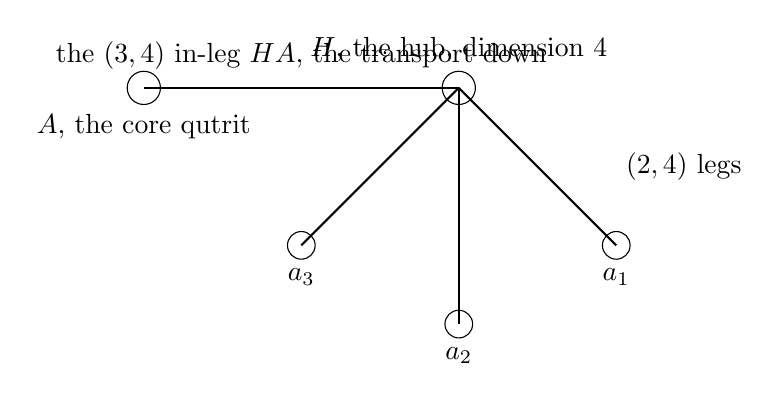
\begin{tikzpicture}[scale=1]
\filldraw[fill=white] (0,0) circle (6pt) node[above=6pt] {$H$, the hub, dimension 4};
\filldraw[fill=white] (-4,0) circle (6pt) node[below=6pt] {$A$, the core qutrit};
\filldraw[fill=white] (2,-2) circle (5pt) node[below=5pt] {$a_1$}; \filldraw[fill=white] (0,-3) circle (5pt) node[below=5pt] {$a_2$}; \filldraw[fill=white] (-2,-2) circle (5pt) node[below=5pt] {$a_3$};
\draw[thick] (-4,0) -- (0,0); \draw[thick] (0,0) -- (2,-2); \draw[thick] (0,0) -- (0,-3); \draw[thick] (0,0) -- (-2,-2);
\node at (-2,0) [above=3pt] {the $(3,4)$ in-leg $HA$, the transport down};
\node at (2,-1) [right] {$(2,4)$ legs};
\end{tikzpicture}\caption{The electron hub with its (3,4) in-leg to the core qutrit and its three (2,4) legs; the block is the hub read transported down the in-leg against the core read, and at the hub letters beyond Z it is cut at the leg $a_3$.}\end{figure}
\end{chproof}
\section{The mixing as the overlap Gram of the (3,4) pairings}\label{mod:VI-7-D543182-w-mxog}
\begin{chwall}[The mixing as the overlap Gram of the (3,4) pairings]\label{box:VI-7-D543182-w-mxog:1}
This result is conditional on the results it rests on, the open results among them consumed at their tables at their grades, the composition riding the lowest grade in its chain, and on the readings of its source disclosed at its register. The mixing as the overlap Gram of the (3,4) pairings across the bodies: at every one of the sixteen in-legs of the roster the pairing, the (3,4) pair ket read at the bases, carries the leg read into the hub frame, and the Gram of the pairings across the roster at one hub letter is the (3,3) overlap of the two core letters at every one of the eighty blocks, the hub frame dropping out at eighty of eighty; washed at the shared qutrit by the group it equals the quark-mixing-block entry cell for cell at seven of sixteen of the core-letter pairings at the plain reading, the pairing against the pairing, and at sixteen of sixteen at the conjugate reading, the first pairing read as the bra, the washed-overlap entry at sixteen of sixteen and the sink-basis entry at four of sixteen at the plain reading; the lepton-side open results re-met; the argument of every entry an exact twenty-fourth root at 600 of 720; so the face read is the second at the first parting, the Gram block of the pairing at the electron in-leg against the pairing at the muon in-leg at the core letters X against Z at every hub letter, washed at the shared qutrit: against the quark-mixing-block entry the Jarlskog element reads minus one ninth and one eighteenth at the Gram where the entry reads one ninth and minus one eighteenth, the block parting at the sign while the cells agree at 107 of 128; the second cell, the conjugate reading at the same block, reads the entry equal.
The first face, the mixing blocks the overlap Gram at every body with every block equal at every compared cell against the quark-mixing-block, washed-overlap and sink-basis entries and the lepton-side controls the same, reads no at the face cell, the blocks equal at seven of sixteen, sixteen of sixteen and four of sixteen; the second face, the first block parting named with both cells, reads yes at the Gram block of the electron pairing against the muon pairing at the core letters X against Z. Open is the sorting of the overlap: read as the bra against the ket, the conjugate reading of the conjugate-letter theorem, the Gram is the quark block cell for cell, and read as the ket against the ket it parts at the sign of the Jarlskog element at the first mixing pairing beyond the Z row.
\end{chwall}
\chstanding{an open result}
\chdeps{Definitions 1.1 to 1.6 and Theorem 166.1 and Open results 166.2 and 166.3}{no theorem beyond it at this release}
A (3,4) pairing at an in-leg carries the core read of the qutrit into the frame of the hub, and two pairings that meet at one hub frame, say the electron in-leg and the muon in-leg, overlap. Because the hub frame drops out, that overlap is the (3,3) overlap of the two core letters whatever the hub letter, and washed at the shared qutrit it is a three by three block whose entries are twenty-fourth roots of unity or zero. The question is whether this Gram across the bodies is the quark mixing block of the foregoing entry. It is, cell for cell at every core-letter pairing, when the first pairing is read as a bra, the sorting the conjugate-letter theorem prescribes, and it parts at the sign of the Jarlskog element when both pairings are read as kets; the open result names that first parting and lays neither reading.
\begin{chbridge}
The quark mixing matrix is the overlap of the bases that diagonalize the up-type and the down-type mass matrices, a unitary three by three matrix whose rephasing-invariant content is the Jarlskog invariant, and its complex conjugate describes the antiquarks \cite{Cabibbo1963,Jarlskog1985}. The correspondence is by name.
\end{chbridge}
\begin{chproof}[finite computation with its exact part]
The premises of this derivation are the axiom and the six definitions of chapter~\ref{mod:FRAMEWORK}, the mixing as the washed overlap and the CKM block of the present chapter, an open result, the mixing blocks at the (3,4) legs of the present chapter, an open result, the records, reads and the Born count of chapter~\ref{mod:I-3-records-reads-and-the-born-count-the-gain-lemma}, a theorem, and the hub step of chapter~\ref{mod:VI-1-hub-step-as-the-weak-interaction}, a theorem. The chain of premises runs back to the axiom through those chapters, and the longest such chain in this compendium is twelve chapters long.
\textit{The object.} The roster is the sixteen in-legs, thirteen at the five bodies with the tau sink as the tau and the tau web of the library beside, each a (3,4) link from a core qutrit to a hub ququart. The pairing at an in-leg and a letter pair, the core letter at the qutrit against the hub letter at the ququart, is the three by four matrix of overlaps of the leg rays with the four transported hub members, equal to the leg-register overlaps of the mixing-blocks entry at twenty of twenty pairs. The figure draws two in-legs meeting at one hub frame.
\textit{The procedure.} Read the rows of each pairing as unit rays through the hub frame. For each pair of in-legs and each pair of letter pairings at one hub letter, form the Gram of the rows of the first pairing against the rows of the second, 400 pairs of letter pairings and eighty designated blocks at one hub letter at both pairings. Wash each block at the shared qutrit by the group. Compare every block cell for cell, in the frozen cell order, against the quark-mixing-block entry, the washed-overlap entry and the sink-basis entry, at the plain reading, the pairing against the pairing, and at the conjugate reading, the first pairing as the bra.
\textit{The smallest instance.} Since the hub frame drops out, every one of the eighty blocks equals the (3,3) overlap of its two core letters, eighty of eighty. At the electron in-leg against the muon in-leg at the core letters X against Z the washed block carries the Jarlskog element
\begin{equation} J_{\mathrm{Gram}} = \big(0,\ 0,\ -\tfrac{1}{9},\ 0,\ 0,\ 0,\ \tfrac{1}{18},\ 0\big), \qquad J_{\mathrm{entry}} = \big(0,\ 0,\ \tfrac{1}{9},\ 0,\ 0,\ 0,\ -\tfrac{1}{18},\ 0\big), \end{equation}
in the eight coordinates of the ring, parting at the sign, the cells agreeing at 107 of 128 at this open result over the pairings; at the conjugate reading the same block reads $J = (0, 0, \tfrac{1}{9}, 0, 0, 0, -\tfrac{1}{18}, 0)$, equal to the entry. Over the sixteen core-letter pairings the plain reading equals the quark-mixing-block entry at seven of sixteen, the washed-overlap entry at sixteen of sixteen and the sink-basis entry at four of sixteen, and the conjugate reading equals the quark-mixing-block entry at sixteen of sixteen. Every entry of the eighty blocks is an exact twenty-fourth root or zero, 600 roots and 120 zeros of 720, and the phase group of the plain washed Z against X block has order three at the generator the eighth power of the twenty-fourth root; the mixing-phase open result is re-met at its composition cells.
\textit{The check.} The counter-tests alter the construction singly and read what moves. Striking a body moves the roster to fifteen in-legs and the first parting. Reading the (2,4) pairings in place of the (3,4) gives blocks of shape two by two and moves the first parting. Leaving the Gram unwashed moves the Born of the conjugate pairings off the flat value. Swapping the ends, the columns as the unit rays, gives blocks of shape four by four. Striking the text unmeets the gate. Each alteration moves the cells it names, five of five. The result was reproduced by an independent route, two engines built apart, equal at every cell, with the seventeen controls the same.
\chcert{80}
\begin{figure}[h]\centering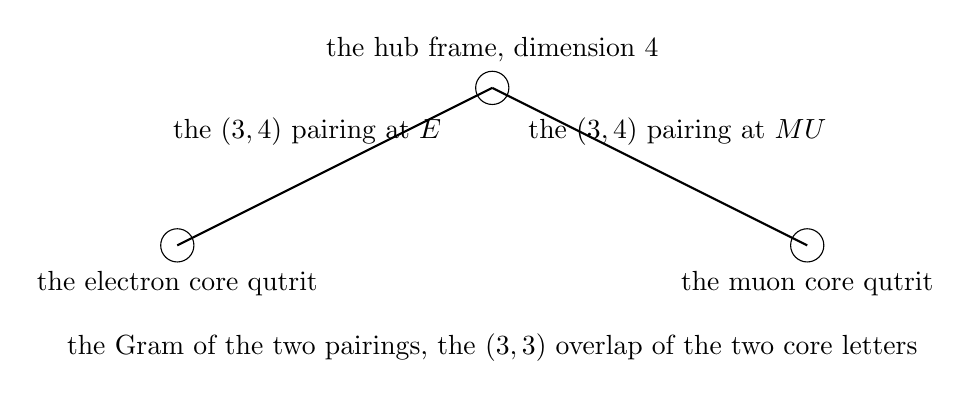
\begin{tikzpicture}[scale=1]
\filldraw[fill=white] (0,0) circle (6pt) node[above=6pt] {the hub frame, dimension 4};
\filldraw[fill=white] (-4,-2) circle (6pt) node[below=6pt] {the electron core qutrit};
\filldraw[fill=white] (4,-2) circle (6pt) node[below=6pt] {the muon core qutrit};
\draw[thick] (-4,-2) -- (0,0); \draw[thick] (4,-2) -- (0,0);
\node at (-2,-1) [above=4pt, xshift=-10pt] {the $(3,4)$ pairing at $E$};
\node at (2,-1) [above=4pt, xshift=10pt] {the $(3,4)$ pairing at $MU$};
\node at (0,-3) [below] {the Gram of the two pairings, the $(3,3)$ overlap of the two core letters};
\end{tikzpicture}\caption{Two (3,4) pairings meeting at one hub frame; their Gram is the (3,3) overlap of the two core letters whatever the hub letter, washed at the shared qutrit.}\end{figure}
\end{chproof}
\par\medskip\noindent{\itshape The mixing read, the next chapter turns to the process the weak sector is known for, beta decay.}\label{narr:close:6-7}\par
\section{Beta decay and the boson widths}\label{mod:VI-8-beta-decay-and-the-boson-widths}
\chdesig{8-8}{6-8}{VI-8-beta-decay-and-the-boson-widths}{VI-8-beta-decay-and-the-boson-widths}
\label{narr:open:6-8}Theorem~170.1 reads beta decay as the release at the plus-two arm and Open result~170.2 the boson widths as the hub-leg genre reads, both open results resting on the hub step and on the decay chapters of Part XII.
\begin{chtheorem}[Beta decay as the release at the plus-two arm]\label{box:VI-8-beta-decay-and-the-boson-widths:1}
Beta decay is read as the release at the plus-two arm at the literal closure reading of the decay graph: at that reading the catalogued neutron web is a non-sink carrying its dock edge at the plus-two arm, and the hub transfer at the dock of the arm, the hub unit of the released body attached at the dock by its in-leg together with the kept-leg hub at the same dock, adds with its end the cross-core object of the released body by an explicit isomorphism at dimensions and links, read through the hub at the order two of its (2,4) in-leg with the dressing of that link at both dressing readings, the readout 2916 at the hub spelling and the cell 1296 over 17689 at both spellings, so the beta rate cell is an output of the rate law at a non-sink. The two partings of the previous open result are closed at this reading: at the stop condition of the pairing move the neutron carried no forward edge, and the object the dock move added, a dock of one site at one link of measure 6, parted from the released body and from the cross-core object; at the literal closure reading the forward edge is present and the hub transfer adds the cross-core object, while the dock move of the previous reading remains the first admitted edge at the dock at which the release parts, its object a dock, printed beside; the deciding table is re-derived in Lean.
\end{chtheorem}
\chstanding{theorem, built at the literal closure reading}
\chdeps{Definitions 1.1 to 1.6, Theorem 158.1 and Open result 158.2, Theorem 203.1, Open result 203.2, Theorem 203.3, Open result 203.4, Theorem 203.5 and Open result 203.6 and Theorems 206.1 to 206.4}{no theorem beyond it at this release}
The box asks whether the rate law of this compendium, which assigns a rate to every unstable web, assigns one to the neutron. It does not, because the neutron is stable at the stop condition the decay graph uses, and the one move that acts at its plus-two arm adds a different object from the one a decay should release.
\begin{chwall}[The boson widths as the hub-leg genre reads]\label{box:VI-8-beta-decay-and-the-boson-widths:2}
The widths of the bosons are read as the hub-leg genre reads: the W and the Z bodies are sinks at the stop condition of the decay graph, so at the primary reading their widths are outputs of the rate law at neither, while at the two readings beside the carriers are non-sinks at all three with their widths defined at all three, the W and the Z at 270 over 49 each and the Higgs at 121 over 16.
\end{chwall}
\chstanding{open result, built and not closed}
\chdeps{Definitions 1.1 to 1.6, Theorem 158.1 and Open result 158.2, Theorem 203.1, Open result 203.2, Theorem 203.3, Open result 203.4, Theorem 203.5 and Open result 203.6 and Theorems 206.1 to 206.4}{no theorem beyond it at this release}
The second box does for the W, the Z and the Higgs what the first does for the neutron, at the stop condition the two carriers are stable and have no width, and only at the readings that admit every forward edge do all three decay, with exact widths and the W and Z widths equal.
\begin{chbridge}
What this chapter calls the release at the plus-two arm the literature calls the beta decay of the neutron and the dock edge its charged-current vertex. The correspondence is by name, and no width and no rate is displayed in this chapter.
\end{chbridge}
\begin{chproof}[finite computation]
The premises are the hub step as the weak interaction of chapter 6-1, an open result, the decay as the forward edge of a non-sink of chapter 9-1 and the rate as the washed square of the read of chapter 9-2, theorems. The chain from the axiom to this chapter is seven chapters long. The procedure of the first box, the input is the neutron web rebuilt from the seeds of the proton web with the arm turned down, 13 sites, 16 links, the measure 133, the hubs $H$ and $F$ at the hub rule, the dressing 81, the first power at the hub spelling and at the dock spelling
\begin{equation}
10773 = 133 \cdot 81, \qquad 133 ;
\end{equation}
the enumeration lists the forward edges of the neutron at the stop condition of the decay graph (none, the neutron a sink as the proton seed is) and the dock edges at the arm at the literal closure reading (two, the dock kind). The test is whether a forward edge of the construction leaves the neutron. The aggregation is the rate by the rate law, the readout of the dock move the measure it adds, 6, multiplied by the dressing. The smallest instance is the one dock edge at the arm, the readout 486 at the hub spelling and 6 at the dock spelling, the washed square 236196, and the rate cell in ticks
\begin{equation}
\Bigl(\frac{486}{10773}\Bigr)^{2} = \Bigl(\frac{6}{133}\Bigr)^{2} = \frac{36}{17689}
\end{equation}
at both spellings, the dressing canceling, and 72 over 17689 over the dock kind of two edges. The object the dock move adds is a dock of one site at one link, of measure 6, against the released object of the construction (four sites at the measure 28) and the cross-core object, parting at every reading. Of the four clauses of the first face, the forward edge of the construction reads no, the dock edge yes, the readout defined yes and the object the cross-core object no.

The procedure of the second box, the inputs are the three carriers, the W word, the Z word and the Higgs word, at their cataloged webs. The enumeration lists their forward edges at three readings, the stop condition of the decay graph, the literal closure and the forward-edge reading, every forward edge rebuilt from its token at the cataloged anatomy with the readout equal to the genre sum at 7 of 7 and at 39 of 39 over every carrier and the top. The test is whether the carrier is a non-sink. The aggregation is the width, the rate law summed over the forward edges. At the stop condition the carriers are non-sinks at 1 of 3 and the widths defined at 1 of 3, the first parting the W word. At the two readings beside the carriers are non-sinks at 3 of 3 with the widths
\begin{equation}
\frac{270}{49}, \qquad \frac{270}{49}, \qquad \frac{121}{16}, \qquad \frac{121/16}{270/49} = \frac{5929}{4320},
\end{equation}
the W over the Z one. The first powers re-met at 9 of 9 and the rate-row cells at 4 of 4.

\emph{Check.} At the neutron the muon cells of the rate law stand beside as the model of a rate at a non-sink, its first power 963 and its washed rate 34958 over 11449. At the carriers the counter-tests at their pinned letters 5 of 5 at the first and the controls the same at both routes but one at the first, a route writing a warning at every piece with every cell equal across the two. Each result was reproduced by an independent route, two engines at every capture byte for byte.
The beta rate as an output of the rate law is supplied by no cataloged non-sink at the stop condition, and the widths of the carriers stand at that reading undefined. Alpha decay is the matter of chapter 9-5.
\chcert{39}
\end{chproof}
\label{chend:VI-8-beta-decay-and-the-boson-widths}
\par\medskip\noindent{\itshape The results of the sector are gathered in the table of the next chapter.}\label{narr:close:6-8}\par
